%************************************************************************* %
%**************************  MODELO TCC UEL  ***************************** %
%************************************************************************* %

%****************************** CLASSE *********************************** %

\documentclass[12pt, openright, oneside, a4paper, english, brazil]{abntex2}   % Padrão Abntex2
		 % openright: capítulos começam em pág ímpar
		 % twoside: para impressão em verso e anverso.

%***************************** PACOTES *********************************** %
%\usepackage[within=none]{newfloat}
\usepackage[utf8]{inputenc}		     % Codificacao do documento (conversão automática dos acentos)

%	DEEL
\usepackage{DEEL}               	 % personalização da ABNTEX2 para a Universidade Estadual de Londrina

%	Fonte
\usepackage[T1]{fontenc}		   	 % Selecao de codigos de fonte.
\usepackage[brazil]{babel}
\usepackage{lmodern}			     % Usa a fonte Latin Modern

%	Matemático e Gráfico
\usepackage{float}
\usepackage{graphics,graphicx}	     % pacotes para inserir figuras .eps ou .jpg
\usepackage{amssymb}           		 % pacote para fontes e simbolos matemáticos
\usepackage{longtable}          	 % possibilita inserir grandes tabelas
\usepackage{color,colortbl,multirow} % permite textos e tabelas com cores
\usepackage{amsmath}           		 % pacote para equações
\usepackage{epstopdf}
\usepackage{ragged2e}
\usepackage{listings}
%\lstset{numbers=left, numberstyle=\tiny, stepnumber=1, numbersep=5pt, basicstyle=\scriptsize ,frame=tbrl}
\usepackage{etoolbox}
%\usepackage{caption}
\usepackage[position=b,singlelinecheck=on]{subfig}

\floatstyle{plaintop}
\newfloat{quadro}{htbp}{loq}
\floatname{quadro}{Quadro}

\makeatletter
\patchcmd{\listof}% <cmd>
{\float@listhead}% <search>
{\@namedef{l@#1}{\l@table}\float@listhead}% <replace>
{}{}% <success><failure>
\makeatother

%\makeatletter
%\renewcommand*{\float@listhead}[1]{%
%	\@ifundefined{chapter}{%
%		\section*{#1}%
%		\addcontentsline{toc}{section}{#1}%
%	}{%
%	\chapter*{#1}% 
%	\addcontentsline{toc}{chapter}{#1}%
%}%
%\@mkboth{\MakeUppercase{#1}}{\MakeUppercase{#1}}%
%}
%\makeatother




%\DeclareFloatingEnvironment{quadro}[Quadro][Lista de quadros]
%\DeclareCaptionType{quadro}[Quadros][Lista de quadros]


% % % % % % % % % % % % % % % % % % % %

\definecolor{codegreen}{rgb}{0,0.6,0}
\definecolor{codegray}{rgb}{0.5,0.5,0.5}
\definecolor{codepurple}{rgb}{0.58,0,0.82}
\definecolor{backcolour}{rgb}{0.95,0.95,0.92}

\definecolor{verde}{rgb}{0,.5725,0.247}

\lstdefinestyle{mystyle}{
	backgroundcolor=\color{backcolour},   
	commentstyle=\color{codegreen},
	keywordstyle=\color{magenta},
	numberstyle=\tiny\color{codegray},
	stringstyle=\color{codepurple},
	basicstyle=\footnotesize,
	breakatwhitespace=false,         
	breaklines=true,                 
	captionpos=b,                    
	keepspaces=true,                 
	numbers=left,                    
	numbersep=5pt,                  
	showspaces=false,                
	showstringspaces=false,
	showtabs=false,                  
	tabsize=2
}

\lstset{style=mystyle}

%	Estrutural
\usepackage{url}
\usepackage{threeparttable}     	 % permite a inserção de notas de rodapé nas tabelas
\usepackage{lscape}             	 % orientação de página LANDSCAPE
\usepackage{pifont}             	 % acrescenta símbolos diferentes.
%\usepackage{cmap}					 % Mapear caracteres especiais no PDF	
\usepackage{lastpage}				 % Usado pela Ficha catalográfica
\usepackage{indentfirst}			 % Indenta o primeiro parágrafo de cada sessão.
\usepackage{enumitem}   % numeros romanos



% Pacotes de citações
\usepackage[brazilian,hyperpageref]{backref}	 % Paginas com as citações na bibl
\usepackage[alf]{abntex2cite}	% Citações padrão ABNT

\data{2018}        % Ano de realização

\begin{document}

%---------------------------------------------------------------
%--------- DADOS BÁSICOS DO TRABALHO (Preencher todos) ---------
%---------------------------------------------------------------


\titulo{ ...}   % Título do Trabalho em Português

\tituloingles{Methods of Labeling and improvement of the energy efficiency of the Center of Technology and Urbanism of UEL with focus on 
lighting}   % Título do Trabalho em Inglês

\palavraschave{1.}  % 5 palavras-chave
\keywords{1.}   % 5 key-words

\DEELautor{Gustavo}{Ribas Roesler}                 
% Aluno autor do trabalho

\curso{Engenharia Elétrica}											

\orientador{Prof. Dr. Silvia Galvão Souza Cervantes}              % Professor Orientador membro da banca 

\membrob{Professor Mestre Osni Viscente}   % Professor membro da banca 
\membroc{Professor}   % Professor membro da banca

\local{Londrina}   % Cidade da instituição

%--------------------------------------------------------------------------------------------


\DEELdedicatoria{Dedico este trabalho a todos aqueles que, de alguma forma,\\ auxiliaram para a concretização desta etapa.}  % Texto da Dedicatória (OBS: dedicatória é opcional)
                                    % Caso não queira inserir, deixe em branco ( \dedicatoria{} )

\DEELagradecimentos{.} 
                                   % Texto dos Agradecimentos (OBS: Agradecimentos é opcional)
                                   % Caso não queira inserir, deixe em branco ( \agradecimentos{} )
                                  

\DEELepigrafe{} 
                                   % Texto da Epígrafe (OBS: Epígrafe é opcional)
                                   % Caso não queira inserir, deixe em branco ( \epigrafe{} )


\DEELresumo{..} 
                                   % Texto do Resumo (OBS: Resumo é Obrigatório)

\DEELabstract{} 
                                   % Texto do Abstract (OBS: Abstract é Obrigatório)



%----- Elementos Pré-Textuais--------------------------
\ElementosPreTextuais
% Insere todos os elementos Pré-Textuais listados (capa, folha de rosto, ...)
												% capa                   % Obrigatório
												% folhaderosto           % Obrigatório
												% fichacatalografica     % Obrigatório
												% folhaaprovacao         % Obrigatório
												% dedicatoria            % Opcional
												% agradecimentos         % Opcional
												% epigrafe               % Opcional
												% resumo                 % Obrigatório
												% abstract               % Obrigatório
\
%--------------------------------------------------------------------------------------------
%\newpage
%---- Outros Elementos Pré-Textuais ----
%--------Lista de figuras--------------------------------------------------------------------
\listoffigures*
\cleardoublepage
%--------Lista de tabelas--------------------------------------------------------------------
\listoftables*
\cleardoublepage


%--------Lista de Siglas e Abreviaturas------------------------------------------------------
%----------Lista de Acronimos --------------------------------
\pretextualchapter{Lista de Siglas e Abreviaturas}

%\renewcommand{\baselinestretch}{2} %espaçamento entre linhas (por definicçào, no espABNT é 2)
\begin{tabbing}
xxxxxxxxxxx \= xxxxxxxxxxxxx \kill
\textsc{UEL}            \> Universidade Estadual de Londrina\\
\textsc{ANEEL}            \> Agência Nacional de Energia Elétrica\\
\textsc{SPDA}          \> Sistema de Proteção Contra Descargas Atmosféricas\\
\textsc{CA}            \> Corrente Alternada\\
\textsc{CC}            \> Corrente Contínua\\
\textsc{CC}            \> Corrente Contínua\\

\end{tabbing}
   % (OBS: Elemento Condicionado à Necessidade) 
%                       % Veja modelo no arquivo list_siglas.tex
%--------Lista de Simbolos e Notação --------------------------------------------------------
%\include{list_simbolos} % (OBS: Elemento Condicionado à Necessidade)
%                       % Veja modelo no arquivo list_simbolos.tex
%--------Sumário-----------------------------------------------------------------------------
\cleardoublepage
\tableofcontents*
\thispagestyle{empty}
%--------------------------------------------------------------------------------------------


%----- Elementos Textuais--------------------------
\textual 
\chapter{Introdução}\label{chp:intro}
\vspace{-1.5cm}
\noindent\rule{\columnwidth}{1.2mm}
\vspace{0.1cm}

.
\section{Objetivos}

\begin{comment}
O objetivo desse trabalho é avaliar a instalação de uma usina fotovoltaica conectada à rede na Universidade Estadual de Londrina (UEL), sendo ela localizada ao lado da Farmácia Escola, tomando como base o edital $N^o$ 0217/2017, emitido no dia 25/10/2017. 

Para contextualizar, será apresentado os benefícios desse sistema fotovoltaico, demonstrando seus respectivos impactos: sociais, econômicos e ambientais gerados. 
\end{comment}
  

\section{Objetivos Específicos}

\begin{itemize}
\item Apresentar um estudo de caso de projeto elétrico de um sistema de armazenamento de grãos.
\item Obter o menor custo financeiro do projeto, atendendo qualidade e respeitando todas as normativas. 
\item Análise detalhada de cada etapa do projeto.

\end{itemize}

\section{Estrutura do Trabalho}
\begin{comment}
 Este trabalho está dividido em 5 capítulos. O primeiro capítulo será referente à uma introdução e contextualização do tema abordado, bem como a motivação do trabalho e os objetivos a serem alcançados.

No segundo capítulo será referente à uma revisão bibliográfica abordando os métodos de etiquetagem em geral, e posteriormente, focando no sistema de iluminação, apresentando o conceito de algumas soluções atuais disponíveis no mercado, que possam ser interessantes para possíveis implementações, onde será analisado a viabilidade financeira.

No terceiro capítulo será mostrado o método utilizado para a tomada de dados, bem como as soluções viáveis a serem expostas para uma possível implementação.

No quarto capítulo será mostrado os dados obtidos através das medições para a obtenção da ENCE do sistema de iluminação, bem como, as projeções com as possíveis implementações das soluções adotadas no trabalho.

No quinto e último capítulo, será abordado as discussões e conclusões com base nos dados obtidos, e nas projeções para as soluções encontradas.

\end{comment}


				  % Capítulo 1 - Texto do cap1.tex
%%
\chapter{Fundamentação Teórica}\label{chp:fundament}
\vspace{-1.5cm}
\noindent\rule{\columnwidth}{1.2mm}



\section{O Armazenamento de Grãos}

\subsection{Histórico}

-- Histórico do armazenamento de grãos até os sistemas 

\subsection{Impacto no Brasil}

A agricultura brasileira, é uma das grandes forças da economia no país e esta  se desenvolvendo de forma cada vez mais eficiente. Com o uso da tecnologia no campo, os processos veem se tornando mais inteligentes e assim aumentando ainda mais a produtividade. 

A produção de grãos, principalmente a soja, é o principal commodit comercializado no país, sendo o Brasil um grande consumidor e exportador. Em um mercado gigantesco e globalizado, este "simples grão" movimenta e influência de formas direta ou indireta a agroindústria como um todo, movimentando bilhões de dólares anualmente. O Brasil é o segundo maior produtor de soja do mundo, em 2017 produziu cerca de 117,208 milhões de toneladas \cite{embrapa}. Mesmo com o aumento da tecnologia a produção ainda é dependente do clima e dos intemperes

% comentar volatilidadee de produção e preço

Com um volume de produção tão grande e um mercado volátil e internacional a necessidade de armazenamento dos grãos se mostra evidente. Caso realizado da maneira correta  este processo pode, além de preservar a matéria prima, aumentar seu valor econômico através dos processos de limpeza e secagem. Conseguindo um produto de maior qualidade e com a possibilidade de  ser comercializado em um momento favorável do mercado, não tendo que ser feito necessária mente no momento da colheita.




\subsection{Sistema a Granel}

O Sistema de armazenamento mantém a matéria prima in-atura, os grãos são recebidos por caminhões e despejados a partir de uma rampa. Através de elevadores de caneca esses grãos são levados ao sistema de pré limpeza, este é o filtro do sistema, faz a separação  . A primeira etapa é no sistema de pré limpeza, através d fazendo uma uma pré limpeza, seleção, secagem e armazenamento do mesmo. 
A primeira etapa é o descarregamento, realizado por caminhões de forma que o grão cai em uma espécie de (bacia) no subsolo e é levado por um elevador de caneca para a pré limpeza.  



-- etapas e sistema
-- implementação - diferentes capacidades - cooperativas. 
-- impacto na economia 


\section{Instalações Elétricas}

\subsection{Normas para Projetos}
Todo projeto deve ser elaborado com base nos documentos normativos, sendo que no Brasil estes são de responsabilidade da Associação Brasileira de Normas e Técnicas (ABNT). Para cada etapa do projeto a sua respectiva norma deve ser consultada. Tendo assim como base geral para este projeto:
\begin{itemize}
\item NBR-5410 Instalações elétricas de Baixa tensão;
\item NBR 5419 Proteção de estruturas contra descargas atmosféricas.
\end{itemize}


% - levantamento de cargas 
\subsection{Motores} 

Os motores  elétricos podem ser definidos como uma máquina que transforma energia elétrica em energia mecânica. 

(Trataremos sobre os motores neste trabalho apenas de maneira simples, não sendo estudado  sobre seu funcionamento mais a fundo.) precisa? 
São divididos em duas principais categorias, os que trabalham a partir de uma fonte de corrente contínua(CC) ou  alternada (CA).

-----subdivisões 

Os motores mais utilizados hoje na indústria, são os de indução trifásicos com rotor em gaiola, sendo considerados mais viáveis financeiramente. Por ter uma alta gama de aplicações, simplicidade de construção, uma longa vida útil e principalmente um  custo reduzido tanto para a compra quanto para a manutenção. (Mamede) . (Franchi)  %/cite

O motor com Rotor em gaiola tem seu funcionamento baseado em três enrolamentos instalados no estator diretamente na fonte de alimentação, sendo que tanto os enrolamentos são deslocados de 120 como a fonte de alimentação trifásica também são defasadas no tempo de 120. A velocidade angular do campo magnético girante é  definida apenas pela frequência da alimentação. (mamede) %\cite 
Assim, se conectado diretamente a rede terá uma velocidade angular fixa.


%Sendo os mais indicados para potências acima de 2 kW, abaixo é justificado o uso de motores de corrente contínua na relação de custos
%definir o motor de gaiola de esquilo (apostila weg)

Dentro do sistema de armazenamento de grãos os motores são utilizados em todas as etapas.
Desde a a pré limpeza, esteiras, elevadores, ventilação até a aeração. Para um bom funcionamento de cada fase, os motores corretos devem ser utilizados, devendo ser  dimensionados  corretamente, atendendo a capacidade  necessitada. 



\subsubsection{Características dos Motores Trifásicos}

Para um uso adequado e otimizado dos equipamentos, é necessário conhece-los como um todo, seu funcionamento e suas principais características. Só com uma análise completa é possível utilizar todo o potencial de uma máquina, minimizando os custos e perdas.

\subsubsubsection{Potência Nominal e Fator de Serviço}

A potência  pode ser definida como a relação entre a energia gasta para realizar determinado trabalho e o tempo em que o mesmo foi executado. A potência nominal de um motor é a potência que o motor pode fornecer no eixo, em regime contínuo, sem elevar os limites de temperatura, da sua classe de isolamento, além do estipulado por norma.

A medida que são aplicadas cargas que fazem o motor trabalhe  muito acima da potência para qual foi projetado a temperatura do motor se eleva além do normal, o que acarreta na redução da vida útil ou mesmo podendo danificar o enrolamento interno do motor chegando a resultar em um curto circuito, e assim a queima do equipamento. (Mamede) %/cite

% Cada motor tem sua rotação nominal, que é a rotação do eixo do motor trabalhando com a sua carga nominal. É chamado de regime de serviço o modo em que o motor opera, sendo que alguns motores trabalham continuamente e outros são acionados de tempos em tempo, oscilando entre estarem parados até mesmo em trabalhar com sobrecarga. (Franchi)  %/cite 
O motor é fabricado para poder trabalhar em uma potência acima da potência nominal, em condições desfavoráveis. Este fator aplicado à potência nominal (uma "folga" do motor) é chamado de fator de serviço, sendo definido como a capacidade de sobrecarga contínua que o motor pode suportar. Como exemplo um motor com fator de serviço de  1,15 pode trabalhar com carga 15\% acima da nominal.  (Franchi)  %/cite


\subsubsubsection{Rendimento}
O rendimento de um motor é a relação entre a potencia ativa fornecida pelo motor(potencia de saída) e a potencia ativa solicitada pela rede (potencia de entrada), sendo quantificado pela equação \ref{eq: rendimento}(Franchi)  %/cite 
 

\begin{equation}
\eta = \frac{P_{saída}}{P_{entrada}}
\label{eq: rendimento}
\end{equation}

Tendo um melhor rendimento com $\eta$ mais próximo de 1. Quanto maiores as perdas do motor, menor é a sua potência fornecida e assim menor é o rendimento.
O resultado vem de dois tipos de rendimentos, do motor: em função da sua potência nominal e em função da potência no seu eixo.  Tendo que o rendimento da máquina aumenta com o funcionamento do motor estando mais próximo da sua potência nominal. (Franchi)  %/cite 
Diversas perdas podem causar diminuição de rendimento, estas serão citadas adiante. 
Uma prática do projetista que pode auxiliar no rendimento do motor é o seu dimensionamento adequado, utilizando o motor de  potência ideal para o uso específico.



\subsubsubsection{Perdas no motor}

Durante o processo de trabalho do motor são geradas diversas perdas, a principal, é a perda por efeito Joule, que ocorre pela dissipação de calor, energia que não é transformada em trabalho. 
%(descrever tipos de perdas, causas e como minimizar) %


\subsubsubsection{Plaqueta de identificação e projetos}

Para facilitar a utilização e manutenção dos motores eles possuem uma plaqueta de informações. Contendo informções necessárias sobre os motores. 

-- colocar imagem 

-- citar cada item




\subsubsection{Partida de Motores}

Existem diversos tipos de partidas de motores, cada uma com suas características vantagens e desvantagens. É de extrema necessidade utilizar a partida mais adequada para o motor, dentro da sua aplicação, podendo economizar principalemte no consumo de energia e desgaste do motor. Será comentado sobre alguns méodos de partida de motores, seu funcionamento e vantagens e desvantagens.

\subsubsubsection{Partida Direta}

O método mais simples de se partir um motor é através da partida direta, onde é conectado as três fases da rede diretamente no motor. Tem a corrente de partida diretamente proporcional a tensão de alimentação e diminui a medida que a velocidade aumenta. 
A partida direta possui certas vantagens, simplicidade de instalação, baixo custo, um conjugado de partida elevado e uma partida rápida. Como desvantagens tem a necessidade de superdimensionamento de cabos(aumentando o custo nessa área), um pico elevado de corrente durante a partida e uma acentuada queda de tensão, podendo interferir em outros equipamentos conectados a rede o que dificulta a partida simultânea de dois ou mais motores de alta potência. Devido a estas características a partida direta no meio industrial é permitida pelas concessionarias apenas para motores de até 10cv. (Franchi)  %/cite

\subsubsubsection{Chave Estrela-Triangulo}
A chave Estrela-Triangulo em comparação com a partida direta tem os efeitos causados pela partida suavizados. Porém, tem a limitação de poder ser utilizada apenas para o sistema de alimentação de seis terminais de dupla tensão nominal: 127/220, 220/380 V ou 380/660 V.
Seu funcionamento se baseia na utilização das duas conexões com o motor. Como o maior pico de corrente de um motor acontece durante a sua partida, o motor inicia conectado na configuração estrela, onde a corrente é reduzida em 1/3 da nominal. Permanece nessa configuração até alcançar uma velocidade próxima da velocidade de regime alternando e então alterna para a conexão em triangulo com a qual trabalha durante todo seu funcionamento.
Além da redução da corrente de partida a chave estrela-triângulo não tem uma queda de tensão elevada durante a partida, não possui limite de manobras e tem custo reduzido. Porém, como desvantagem trás a necessidade dos seis terminais e a dupla tensão e o conjugado de partida reduzido de 1/3 do nominal, inviabilizando a partida em aplicações que necessitam alto conjugado já na partida. (Mamede) %cite 


\subsubsubsection{Softstarter}
Diferente dos outros tipos de partidas, a soft-starter ou partida estática, possuí um circuito eletrônico acoplado a um
microprocessador, que controla tiristores colocados em paralelo, 2 a 2 em cada fase da rede.

Assim que o motor é acionado, o sistema controla a tensão eficaz que entra nos terminais, com a variação do ângulo dos tiritosres. A tensão é aumentada gradativamente de forma linear (uma rampa), minimizando os picos de corrente e permitindo que o motor parta de forma suave. 
Essa partida suave trás diversas vantagens, como uma baixa interferência na tensão da rede, um menor gasto de energia e aumento da vida útil do motor, pois tem aumento gradativo também do conjugado na partida, também protege o motor contra aquecimentos vindos de sobrecargas ou partidas frequentes e na  detecção de desequilíbrio e falta de fase. Um único equipamento pode ser utilizado para partir mais de um motor.  (MAMADE e flich) %cite
Apesar de um custo mais elevado em comparação às outras partidas, a softstarter compensa seu custo em muitas aplicações, principalmente para motores de potência elevada, podendo até ser considerada uma necessidade necessidade.

O equipamento possui uma interface de interação homem/máquina, onde pode ser ajustado os valores de tensão inicial de partida, que é responsável pelo conjugado inicial que irá acionar a carga, e o intervalo de tempo que leva para alcançar a tensão de linha do sistema.



Na análise de tensão durante esse intervalo de tempo tem-se uma rampa e após uma tensão constante.


\subsubsubsection{Comparação de corrente de partida}
Além dos métodos citados existem muitos outros, como autotransformador, chave compensada %

\subsubsection{Proteção de motores}
Os motores são a ferramenta final das aplicações e acarretam no maior impacto financeiro, considerando a parte elétrica de uma obra, portanto, devem estar bem dimensionados e protegidos contra os impactos que possam causar danos ou até a perda dos motores. Abaixo é citado alguns impactos que podem causar danos aos motores:  
\begin{itemize}
\item Sobrecargas ;
\item Curto-circuitos;
\item Desequilíbrio, ausência ou inversão de fases;
\item Falta de isolação entre espiras;
\item Sub e sobretensão;
\item Partidas incompletas ou frequentes;
\item Rotor bloqueado;
\item Subcorrente. 
\end{itemize}


Dentre tantos itens que podem causar danos ao motor, diferentes tipos de proteção são utilizadas para cada possível anormalidade.

--- Descrever os tipos de proteção e dimensionamento.

% SOBRECARGA A sobrecarga nos motores elétricos é causada pela solicitação de uma potência mecânica superior a sua capacidade nominal. Nestas condições, há um aumento na corrente absorvida da rede. Consequentemente ocorrerá um aumento nas perdas totais do motor. Com isso, haverá uma elevação de temperatura, se esse acréscimo de temperatura ultrapassar a classe de isolamento do motor, este poderá ter sua vida útil reduzida. Em se tratando de dispositivos de proteção, estes têm por função desligar o motor em situações de sobrecarga, com o objetivo de manter a temperatura interna dentro dos limites aceitáveis de seus materiais isolantes. 




\subsection{Cabos Elétricos}

emprestar livro que esta com o rafael  de cabos. 

- tipos de cabos elétricos/ pp / cobre / alumínio 
- vantagens e desvantagens
- dimensionamento
- norma tabelas (projeto)

\subsection{Eletrodutos}

--- tipos de eletrodutos
--- cálculo e dimensionamento
--- norma e tabelas (projeto)



\subsection{Iluminação}

----iluminação túnel e externa


\section{Sistema de proteção contra descargas Atmosféricas (SPDA)}

De maneira simplificada as descargas atmosféricas são formadas a partir da diferença de potencial entre a terra(potencial positivo) e nuvem(potencial negativo), quando esta diferença de potencial aumenta a ponto de superar a resistência dielétrica do ar. % cite http://www.inpe.br/webelat/homepage/

Todos os tipos de edificações, estão sujeitas a serem atingidas por descargas atmosféricas. 
Os sistemas de armazenamento de grãos a granel, possuem em sua grande maioria silos de metal, com uma altura considerável chegando a mais de 20 metros, equivalente a um prédio detatatta andares. Caso não estejam devidamente protegidos, os estragos causados podem ser gigantescos, tanto para a estrutura, equipamentos ou até mesmo para a vida humana. Só em Londrina-PR é registrado uma densidade de descargas 4,7345712944 por $\frac{km^2}{ano}$, estando na posição 1758 do ranking nacional. % fonte de densidade de descargas na cidade.  http://www.inpe.br/webelat/homepage/

A fim de evitar essas (catástrofes), em quaisquer edificações deve-se ser utilizado um sistema de proteção contra descargas atmosféricas (SPDA). Para descobrir quão eficiente o sistema deve ser ou qual deve ser utilizado, o primeiro passo é conhecer o chamado fator de risco. Este a partir deste valor é estabelecido uma provável perda anual de bens ou vidas devido a descargas elétricas. A norma NBR-5419 estabelece o nível de risco que uma edificação pode estar de acordo com suas características. O projeto de um SPDA deve ser suficiente para alterar esse fator de risco de forma a enquadrar o nível de proteção desta edificação a norma. 



\subsection{Cálculo do fator de Risco}
Este fator de risco é calculado a partir de vários parâmetros e características do sistema em questão, seguindo a norma NBR-5419

--- descrever o cálculo de fator de risco segundo a norma

\subsection*{Tipos de sistemas de proteção}

Os sistemas de proteção não são projetados para evitar as descargas elétricas que podem atingir a edificação, mas para interceptar estas descargas e fazer com que a corrente elétrica possa fluir para a terra sem causar danos.
São três principais tipos de sistemas bem definidos, podem ser utilizados individualmente ou uma combinação de dois deles ou mesmo os três implementando condutores não naturais na estrutura com a finalidade de proteção contra descargas atmosféricas. Além dos sistemas implementados os SPDA podem utilizar a própria edificação, chamados de condutores naturais as partes integrantes das estruturas que não possam ser alteradas, como pilares e a fundação. 


----- Descrever cada tipo de spda e exemplificar aplicações para cada um


\subsection{Planejamento de Projetos Elétricos}

---- seguir MAMEDE


\begin{comment}




%Para termos uma noção do processo de histórico de evolução do sistema fotovoltaico. Começamos citando o seu primeiro aparecimento, quando  Edmond Becquerel, em 1839, conseguiu produzir uma diferença de potencial mergulhando placas metálicas, de platina ou prata, num eletrólito quando expostos a luz.

%Posteriormente, em 1877, dois inventores norte americanos W. G. Adams e R. E. Day, utilizaram a propriedade fotocondutora para produzir o primeiro dispositivo sólido de produção de eletricidade através da exposição a luz, o qual apresentava uma baixa eficiência, aproximadamente 0,5\%.

%Com o desenvolvimento da ciência no século XX, possibilitou-se o nascimento da célula solar moderna. Em 1953 o químico americano Calvin Fuller, juntamente com o físico Gerald Pearson, produziram uma barra de silício dopado com pequenas concentrações de gálio, o que torna condutor, sendo as carga móveis positivas, conhecidas como silício do tipo-p. Após mergulharem essa barra em um banho quente de lítio, criou-se uma zona com um excesso de elétrons livres, sendo eles conhecidos como silício do tipo-n. \cite{MeioSeculo}

%Uma das primeiras e mais importante aplicações da célula solar ocorreu em 1958, quando o satélite \textit{Vanguard I} foi lançado ao espaço, no qual apresentava seis painéis solares montados no corpo esférico do pequeno satélite para realizarem sua alimentação. \cite{Telescopio}

%Alguns anos mais a frente, em 1973, com a crise do petróleo, surgiu a necessidade de aumentar o investimento em programas de investigação para reduzir o preço de produção das células solares.

%Como resultado desse processo, a eficiência das células solares aumentaram, ultrapassando a barreira dos 20\% pelas células de silício monocristalino da Universidade de New South Wales, na Austrália. \cite{MeioSeculo}

%No Brasil, por volta de 1970, os estudos ligados a energia solar somente acontecia dentro das instituições de ensino, como universidades e centros de pesquisa, por falta de incentivos fiscais não obtiveram importância na matriz energética brasileira. \cite{MeioSeculo}

%Apesar da criação da Associação Brasileira de Energia Sola ocorrida em 1978, e do $1^o$ Simpósio de Energia Solar Brasileira, as pesquisas relacionadas a energia solar se moviam a passos lentos. \cite{ABENS}. 

%Na década de 80 iniciou-se a construção de centrais fotovoltaicas pilotos de médio porte, todas instaladas na Europa e nos EUA. 

%Em 1990, houve a utilização de tecnologia fotovoltaica para a eletrificação rural em países em desenvolvimento, como o Brasil. \cite{CEPEL}. Assim, com o mercado fotovoltaico em desenvolvimento, países começaram a investir nessa tecnologia, como a Alemanha, que em 1999 apresentava um total acumulado de painéis solares que possibilitou atingir o primeiro gigawatt de energia produzida. Com esse contínuo desenvolvimento, em 1998 foi atingida a eficiência máxima recorde de 24,7\% com células em monocristalino.\cite{MeioSeculo}  A partir dessa evolução nota-se aumento dos incentivos políticos e econômicos que fomentaram o crescimento de pesquisas em energias renováveis na maioria dos países, o desenvolvimento da energia solar se intensificou, alimentada pela busca em diversidade energética e a diminuição dos impactos ambientais pelos combustíveis fósseis.

 
\subsection{Políticas de incentivo no Brasil}
Para entendermos a evolução e progressão das políticas brasileiras relacionadas a energia solar, precisamos analisar um pouco do contexto histórico do nosso país.

A instituição responsável por implementar as políticas para a exploração e garantir a qualidade de energia elétrica no Brasil é a Agência Nacional de Energia Elétrica (ANEEL). 

Com o intuito de promover o incentivo a geração de energia distribuída, em 17 de abril de 2012, a ANEEL através da Resolução Normativa no. 482/2012, estabeleceu as condições gerais para o acesso de microgeração e minigeração distribuída aos sistemas de distribuição de energia elétrica.

Pode-se destacar alguns pontos importante dessa Rsolução Normativa, tais como:

\begin{enumerate}[label=\Roman*.]
\item “Microgeração distribuída: central geradora de energia elétrica, com potência instalada menor ou igual a 100 kW e que utilize fontes com base em energia hidráulica, solar, eólica, biomassa ou cogeração qualificada, conforme regulamentação da ANEEL, conectada na rede de distribuição por meio de instalações de unidades consumidoras;
\item Minigeração distribuída: central geradora de energia elétrica, com potência instalada superior a 100 kW e menor ou igual a 1 MW para fontes com base em energia hidráulica, solar, eólica, biomassa ou cogeração qualificada, conforme regulamentação da ANEEL, conectada na rede de distribuição por meio de instalações de unidades consumidoras; 
\item Sistema de compensação de energia elétrica: sistema no qual a energia ativa gerada por unidade consumidora com microgeração distribuída ou minigeração distribuída compense o consumo de energia elétrica ativa.
\end{enumerate}

Através da Resolução Normativa (REN) n$^o$  482/2012 foi criado o Sistema de Compensação de Energia Elétrica, permitindo que o consumidor instale pequenos geradores (assim como painéis fotovoltaicos e microturbinas eólicas) em sua unidade consumidora e troque energia com a distribuidora local com objetivo de reduzir o valor de sua fatura de energia elétrica. \cite{AMBIENTE} 

O Sistema de Compensação de Energia Elétrica consiste quando a quantidade de energia gerada em determinado mês for superior a energia consumida naquele período, o consumidor fica com créditos que podem ser utilizados para diminuir a fatura dos meses seguintes.

Em 2015 houve a REN n$^o$ 687/2015, como atualização da REN n$^o$ 484/2012, na qual estabeleceu novas regras para esses sistemas. O novo prazo de validade dos créditos passou de 36 para 60 meses, sendo que eles podem também ser usados para abater o consumo de unidade consumidora do mesmo titular situado em outro local, desde que na área de atendimento de uma mesma distribuidora.

Uma novidade dessa resolução refere-se a geração partilhada, como sendo a micro ou minigeração distribuída que pode ser instalada em condomínios, ou seja, um empreendimento com múltiplas unidades consumidoras. Assim sendo, a energia gerada dividida entre os condôminos em porcentagens definidas pelos próprios consumidores.

Conforme segue a atualização da resolução do artigo 6$^o$ da ANEEL, o acesso ao sistema de compensação de energia elétrica os consumidores responsáveis por unidade consumidora:

\begin{enumerate} [label=\Roman*.]
\item com microgeração ou minigeração distribuída;
\item integrante de empreendimento de múltiplas unidades consumidoras;
\item caracterizada como geração compartilhada;
\item caracterizada como autoconsumo remoto.
\end{enumerate}
§ Para fins de compensação, a energia ativa injetada no sistema de distribuição pela unidade consumidora será cedida a título de empréstimo gratuito para a distribuidora, passando a unidade consumidora a ter um crédito em quantidade de energia ativa a ser consumida por um prazo de 60 (sessenta) meses.

Com a atualização, algumas regras foram modificadas, como segue abaixo:

\begin{itemize}
\item A microgeração distribuída consiste em uma central geradora de energia elétrica, com potência instalada menor ou igual a 75 kW.
\item A minigeração distruída consiste em uma central geradora de energia elétrica, com potência instalada superior a 75 kW e menor ou igual a 3 MW para fontes hídricas ou menor ou igual a 5 MW para cogeração qualificada.

\end{itemize}

Outro fato importante que marcou o crescimento de energias renováveis para o Brasil foram os Leilões de Energia realizado pelo Governo Federal através das Portarias n$^o$226/2013 e n$^o$300/2013, do Ministério de Minas e Energia. Sendo incluído a fonte solar nos leilões de entrega A-3/2013 e A-5/2013, abrindo possibilidades da fonte solar competir igualmente com outras fontes, como eólicas e térmicas.  

Como resultado do leilão ocorrido no mercado de energia em 2013 no Brasil, as fontes eólica e solar lideraram as inscrições para o ano de 2016. Foram 629 parques geradores de energia eólica e uma oferta de 15042 MW inscritos na Empresa de Pesquisa Energética (EPE). A geração solar totalizou 109 projetos do tipo fotovoltaico, somando uma potência instalada de 2792 MW e sendo ela distribuída pelas regiões: Bahia, Minas Gerais, Paraíba, Piauí e Rio Grande do Norte. \cite{EPE}


\section{Programa Brasileiro de Etiquetagem em Edificações}

Tendo em vista o aprimoramento da eficiência energética em edificações, em conjunto com a crescente popular das soluções sustentáveis, há anos, vem ocorrendo o desenvolvimento de normas e certificações, em diversos lugares do mundo. No Brasil, o Programa Brasileiro de Etiquetagem, vem sendo implantado, desde 2001, através da Lei nº10.295 (BRASIL, 2001a)\cite{Lei}, também chama de Lei de Eficiência Energética, que estimula o desenvolvimento tecnológico, a preservação ambiental e a introdução de produtos mais eficientes no mercado nacional.


Com base no Balanço Energético Nacional (2017)\cite{BEN}, as edificações são responsáveis por cerca de 51\% do consumo energético brasileiro, sendo que 29\% desse consumo é referente às edificações residenciais, 19\% é referente às edificações comerciais e aproximadamente 3\% referentes à edificações públicas. Tendo em vista esses dados, surge a necessidade de reduzir o consumo energético, adotando certas medidas para aprimorar a eficiência energética dessas edificações.

No que diz respeito à edificações, o Brasil possui um regulamento específico para edificações residenciais, o RTQ-R, e outro regulamento para edificações comerciais, de Serviços e Públicas, chamado Regulamento Técnico da Qualidade para o Nível de Eficiência Energética de Edificações Comerciais, de Serviço e Públicas(RTQ-C)\cite{RTQ-C}, o qual será a base deste trabalho, uma vez que será avaliado uma edificação Pública.

\subsection{Regulamento Técnico da Qualidade para o Nível de Eficiência Energética de Edificações Comerciais, de Serviço e Públicas(RTQ-C)}

O Regulamento Técnico da Qualidade para o Nível de Eficiência Energética de Edifícios Comerciais, de Serviços e Públicos (RTQ-C)\cite{RTQ-C}, contém uma série de procedimentos essenciais para poder obter a ENCE do programa Brasileiro de Etiquetagem em Edificações, chamado PBE edifica, que é uma parceria do INMETRO com a procel. A classificação das edificações são do nível A até o nível E, sendo o nível A o mais eficiente, e por consequência, o nível E, o menos eficiente, são baseadas nos critérios desse regulamento.\cite{ManualEE}

Para se ter uma real eficiência energética, os critérios mostrados no RTQ-C devem estar presentes no início do projeto de uma edificação, onde deve-se atender ao maior número de requisitos que o regulamento exige para uma obra.\cite{ManualEE} 

Existem três grupos principais à serem observados, no que diz respeito à Eficiência Energética, que são: Envoltória, Sistema de Iluminação e Sistema de Condicionamento de AR, e para avaliar a Eficiência Energética de uma edificações, cada um desses grupos devem ser avaliados separadamente, sendo atribuído pesos, da seguinte maneira: 30\% para envoltória, 30\% para o sistema de iluminação e 40\% para para o sistema de condicionamento de ar. Vale a pena ressaltar que a envoltória deve ser avaliada integralmente, já os sistemas de iluminação e condicionamento de ar, podem ser avaliados de forma parcial.\cite{ManualEE}

O RTQ-C também prevê bonificações, a qual varia de 0 a 1, podendo acrescentar até um ponto na Classificação Final da Eficiência Energética da edificação. Para se obter essas bonificações, é necessário implementar algumas soluções, sistemas ou equipamentos que, de forma comprovada, proporcionem um aumento na eficiência, ou uma redução no consumo energético da edificação. Sistemas de fontes renováveis de energia, como por exemplo, a instalação de células fotovoltaicas, que utilizam a luz solar para gerar energia, é um exemplo de sistemas que podem gerar bonificações para as edificações.\cite{ManualEE}


\subsection{Como Obter a Etiqueta(ENCE)}


A etiqueta do PBE Edifica é emitida por um Organismo de Inspeção Acreditado (OIA), uma empresa pública ou privada autorizada e reconhecida
pelo INMETRO. O INMETRO disponibiliza em seu site\cite{INMETRO}, uma relação da OIAs que estão disponíveis para realizar as creditações no Brasil.\cite{ManualEE}

A etiqueta do PBE edifica é obtida através de uma OIA, que analisará toda a documentação\cite{Doc} exigida, e classificará os projetos, ou edificações construídas. Vale a pena ressaltar que, essas duas etapas, documentação e classificação, podem ser realizadas por OIAs diferentes, com orçamentos separado.\cite{ManualEE}

Primeiramente, antes de submeter a documentação ao OIA, a pessoa interessada em obter a ENCE deve adotar um dos dois métodos existentes de avaliação da eficiência energética, e esses métodos são: o método prescritivo e o método da simulação. 

O método prescritivo é uma metodologia simplificada, a qual avalia as edificações utilizando equações e tabelas. Esse método observa os requisitos e parâmetros exigidos pelo RTQ-C, analisando os indicadores de consumo de energia, bem como o conforto térmico das edificações. Já o método da simulação compara os parâmetros da edificação proposta tendo em vista um modelo de referência em eficiência energética. Ao realizar a simulação, é avaliado o consumo de energia anual em função das variações climáticas de dos hábitos de uso. O método da simulação é mais flexível que o método prescritivo, e permite incorporar novas tecnologias. A Figura \ref{diagrama_metodos}, mostra um diagrama dos métodos citados.\cite{ManualEE}


\begin{figure}[H]
\centering
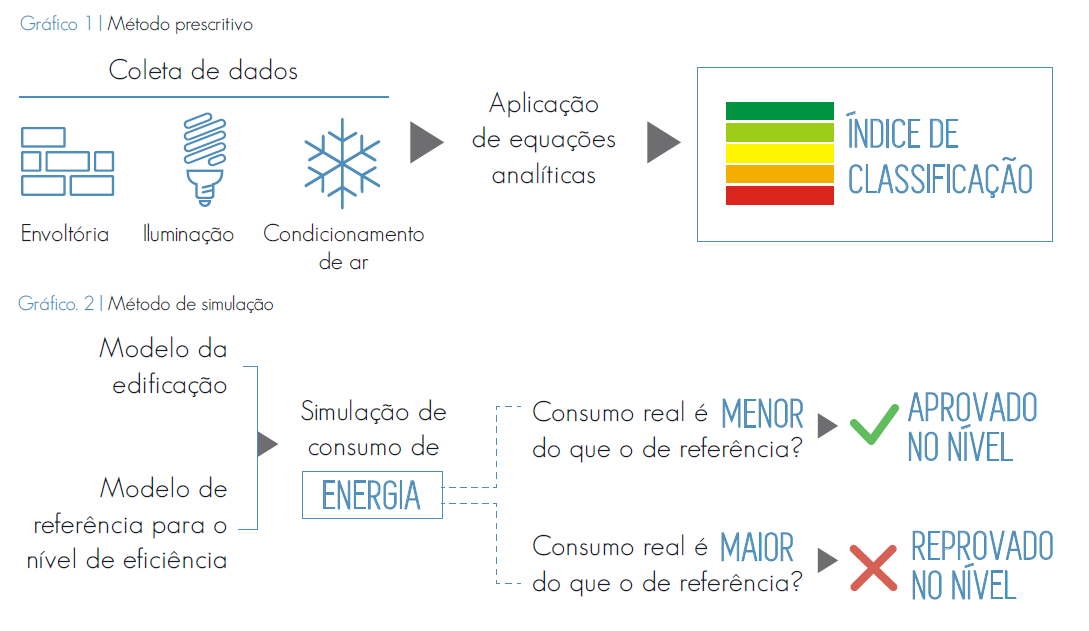
\includegraphics[width = 1\textwidth]{Figuras/diagrama_metodos.PNG}
\caption{Diagrama dos métodos Prescritivo e Simulação.}
\label{diagrama_metodos}
\textbf{Fonte:} LabEEE, Retirado de \cite{ManualEE}.
\end{figure}

Com base no método escolhido, prescritivo ou simulação, o OIA irá realizar a inspeção. Ao término de todo o processo, serão emitidos a ENCE do projeto e o relatório da inspeção. Após a construção da edificação ser concluída, o OIA realizará uma outra inspeção no local, para verificar se as características que foram previamente descritas no projeto, que foi realizada a etiquetagem, foram devidamente atendidas, e então, são emitidos novamente uma ENCE e o relatório de inspeção.\cite{ManualEE}

Existem certos fatores que influenciam no preço de uma etiquetagem, e esses fatores são: tamanho e a complexidade da edificação, o escopo pretendido e o método escolhido, prescritivo ou simulação. Leva-se em conta também, o valor dos custos de logística durante as inspeções do edifício construído. Após receber todas as certificações, essas devem ser expostas em locais visíveis na edificação, seguindo as exigências do regulamento\cite{RTQ-C}.\cite{ManualEE}

Se uma edificação obtém uma ENCE parcial para a envoltória, se torna possível a obtenção de etiquetas parciais para os demais requisitos, ou até mesmo uma etiqueta geral. Se um construtor vende os pavimentos em uma planta que já possui uma ENCE parcial de envoltória, e a empresa, ou o proprietário de um andar inteiro, submete os sistemas de iluminação e de condicionamento de ar, ele obterá uma classificação geral do pavimento. Se nesta mesma edificação, o administrador do condomínio decide submeter apenas o sistema de iluminação das áreas comuns, será obtida uma ENCE com duas etiquetas parciais para estes ambientes: a da envoltória, e a do sistema de iluminação. \cite{ManualEE}


\subsection{Equação matemática para a obtenção da Pontuação Total(PT)}

Para se obter a classificação geral do nível de Eficiência Energética, deve-se levar em consideração os dados fornecidos pelo construtor, e os dados gerados durante a inspeção do OIA, sempre tendo como base o RTQ-C. Gera-se uma pontuação total(PT), calculada com base nos dados da construção, que permite obter o nível da etiqueta, como é mostrado na Figura \ref{etiqueta}.\cite{ManualEE} 


\begin{figure}[H]
\centering
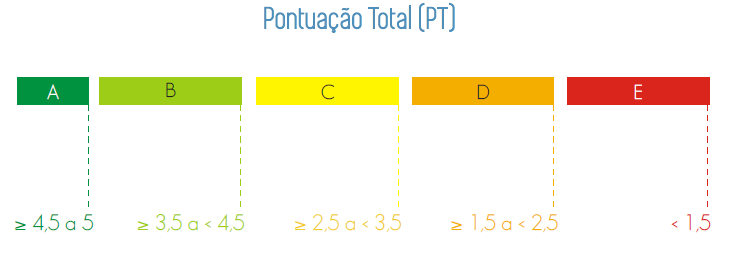
\includegraphics[width = 1.1\textwidth]{Figuras/etiqueta.PNG}
\caption{Nível da etiqueta com base no cálculo da pontuação total.}
\label{etiqueta}
\textbf{Fonte:} Retirado de \cite{ManualEE}.
\end{figure}

A pontuação total é calculada por meio de uma equação, a qual atribui pesos aos sistemas de envoltória, iluminação e condicionamento de ar. Vale ressaltar que se a edificação possuir sistemas de bonificação, como por exemplo, um sistema de energia solar com célula fotovoltaica, acrescenta-se à pontuação um valor de até 1 ponto. A Equação \ref{Eq_PT}, mostra uma soma ponderada desses grupos de requisitos, considerando também as bonificações.\cite{ManualEE}

\begin{equation}
\scriptstyle PT = 0,3 \cdot \{(EqNumEnv \cdot \frac{AC}{AU}) + (\frac{APT}{AU} \cdot 5 + \frac{ANC}{AU} \cdot EqNumV)\} +  0,3 \cdot(EqNumDPI) + 0,4 \cdot \{(EqNumCA \cdot \frac{AC}{AU}) + (\frac{APT}{AU} \cdot 5 + \frac{ANC}{AU} \cdot EqNumV)\} + b_0^1
\label{Eq_PT}
\end{equation} \begin{center}{\textbf{Fonte:} Retirado de \cite{RTQ-C}.}\end{center}


Na Equação \ref{Eq_PT}, tem-se que:

\begin{itemize}
\item EqNumEnv: Equivalente numérico da envoltória;
\item EqNumDPI: Equivalente numérico do sistema de iluminação, identificado pela sigla DPI, de Densidade de Potência de Iluminação;
\item EqNumCA: Equivalente numérico de ambientes condicionados artificialmente;
\item EqNumEnv: Equivalente numérico de ambientes não condicionados e/ou ventilados naturalmente;
\item APT: Área útil dos ambientes de permanência transitória, desde que não condicionados;
\item ANC: Área útil dos ambientes não condicionados de permanência prolongada, com comprovação de percentual de
horas ocupadas de conforto por ventilação natural (POC);
\item AC: Área útil dos ambientes condicionados;
\item AU: Área útil;
\item b: Pontuação obtida pelas bonificações.
\end{itemize}

Pode-se notar que a Equação \ref{Eq_PT} pondera cada um dos requisitos em função das características das áreas úteis totais, do ambientes condicionados e dos ambientes de passagem e de permanência.


\section{Pré-requistos Gerais Para a Etiquetagem}

As edificações que possuem uma certificação de eficiência energética, devem ser capazes de, a qualquer momento, indicar os padrões de consumo, como, onde e em que horas se consome uma maior quantidade de energia elétrica. Só é possível realizar essas indicações com a presença de circuitos elétricos separados por uso final, esse é o primeiro pré-requisito geral para a etiquetagem. Vale ressaltar que existem exceções, como no caso de hotéis, que possuem circuitos integrados por quarto, que se desligam quando estão desocupados. \cite{ManualEE}

O principal consumo de energia elétrica residencial é o sistema de aquecimento de água. Se em uma residência, o chuveiro elétrico representa certa de um quinto do consumo de energia elétrica total, em edificações comerciais, o uso desse aparelho, com grande demanda de água aquecida, como em shoppings, hospitais, entre outros estabelecimentos comerciais, torna inviável realizar a etiquetagem com padrões elevados de eficiência.\cite{ManualEE}

Se a demanda por água aquecida em uma edificação for igual, ou superior, a 10\% do consumo de energia elétrica, o RTQ-C\cite{RTQ-C} prevê a utilização de aquecimento solar, a gás ou por bombas de calor. Para a obtenção da ENCE com nível A, toda a água aquecida, deve ser gerada por essas fontes de energia, e também, deve atender aos requisitos exigidos no regulamento, os quais incluem, o isolamento das tubulações e a existência de reservatórios para preservar o calor. As edificações que possuem um sistema de aquecimento solar e a gás que atendam menos de 70\% da demanda de água aquecida, e que sejam complementados por sistemas elétricos, poderão atingir no máximo o nível C na classificação geral da ENCE.\cite{ManualEE}


\section{Envoltória}

No documento ``EFICIÊNCIA ENERGÉTICA: GUIA PARA ETIQUETAGEM DE EDIFÍCIOS''\cite{ManualEE} disponibilizado pelo Ministério do meio ambiente em conjunto com a Secretaria de Mudanças Climáticas e Qualidade Ambiental e o Departamento de Mudanças Climáticas, é definida a envoltória como sendo:

\begin{quotation}
``A envoltória pode ser comparada à pele da edificação. Trata-se do conjunto de elementos construídos que compõem os fechamentos dos ambientes
internos em relação ao ambiente externo. Todos os elementos que estão acima do nível do solo e com contato com o exterior ou com outro
edifício pertencem à envoltória. Exemplos: cobertura, paredes, fachada e aberturas.''\cite{ManualEE}
\end{quotation}

Para a obtenção da ENCE parcial da envoltória existem três pré-requisitos específicos a serem analisados, os quais são: Transmitância térmica da
cobertura e de paredes exteriores, Cores e absortância de superfícies e Iluminação zenital. A classificação obtida será conforme pode-se observar no diagrama da Figura \ref{diagrama_envoltoria}.



\begin{figure}[H]
\centering
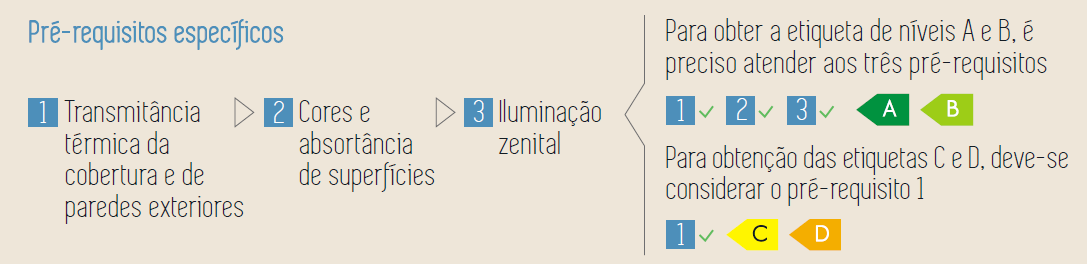
\includegraphics[width = 1.1\textwidth]{Figuras/diagrama_envoltoria.PNG}
\caption{Pré-requisitos específicos da envoltória.}
\label{diagrama_envoltoria}
\textbf{Fonte:} Retirado de \cite{ManualEE}.
\end{figure}

\subsection{Transmitância térmica da cobertura e de paredes exteriores}

As edificações estão sujeitas a constates trocas de energia, através de luz ou calor, entre os meios interior e exterior, e com isso, existem muitos fatores, sejam esses naturais ou artificiais, que podem interferir nesse fenômeno, de transmitância térmica, como por exemplo: materiais de construção, que se comportam de forma distinta para a radiação solar. Afetam também a esse pré-requisito, a existência de fachadas e a maneira como foram construídas.\cite{ManualEE}

Pode-se medir essa troca de energia, conhecida como transmitância térmica, que é uma medida do calor que passa em um intervalo de tempo, por uma área, com base na diferença de temperatura, medido em $W/m^2K$. Existem certos detalhes a serem considerados no cálculo da transmitância térmica. Na Figura \ref{env1}, nas duas primeiras edificações, os planos de vidro externos, por apresentarem superfícies opacas, que no caso geram sombreamento, não são considerados no cálculo da transmitância térmica. Porém, na terceira edificação, mesmo possuindo uma proteção interna, deve ser considerado no cálculo da transmitância térmica. Ou seja, pórticos, proteção solar e outras superfícies opacas, independentemente de estarem atrás dos vidros, contribuem com a redução da entrada de calor.\cite{ManualEE}


\begin{figure}[H]
\centering
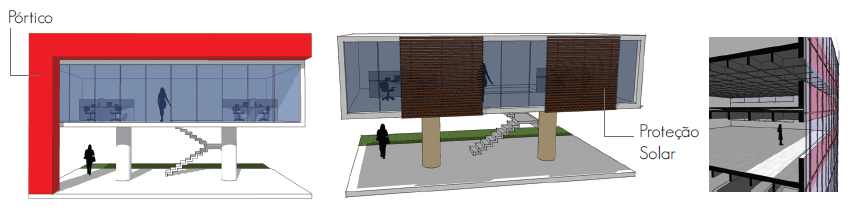
\includegraphics[width = 1.1\textwidth]{Figuras/env1.PNG}
\caption{Edificações para descrever alguns detalhes a serem considerados no cálculo da transmitância térmica.}
\label{env1}
\textbf{Fonte:} Retirado de \cite{ManualEE}.
\end{figure}

Existem mais dois fatores que influenciam diretamente o estudo da transmitância térmica, que são: as zonas bioclimáticas e se os ambientes são
condicionados artificialmente ou não-condicionados. Dependendo da região do Brasil, na qual a edificação será construída, as trocas de energia são muito diferente, e isso interfere diretamente no cálculo da transmitância térmica.\cite{ManualEE}

Já na questão dos ambientes condicionados artificialmente ou não-condicionados, tem-se que, um edifício estará apto a obter a ENCE parcial de nível A, se atender aos pré-requisitos específicos da envoltória, e também, deverá apresentar, nos ambientes de permanência prolongada, os limites de transmitância térmica mais restritivos para ambientes condicionados artificialmente, e nas áreas onde a permanência ocorre de forma transitória, deverá apresentar os limites para ambientes não-condicionados.\cite{ManualEE}

\subsection{Cores e absortância de superfícies}

As cores interferem diretamente na quantidade de radiação absorvida, e portanto, também é um pré-requisito ao avaliar a eficiência energética da envoltória. Simplificadamente, quanto maior for a absortância da edificação, maior será o calor interno da mesma.\cite{ManualEE}

Esse índice de absortância varia conforme as cores e os tipos de tintas utilizados para a pintura das superfícies opacas, as cores claras por exemplo, refletem melhor a luz para dentro da edificação, já utilizando cores escuras, não se terá uma boa reflexão da luz para o interior do edifício. As cores utilizadas nas pinturas do telhados também influenciam, ou seja, telhados pintados com cores claras podem aumentar a luz que as aberturas zenitais transmitem. Pode-se obter esse índice de absortância dos fabricantes de tinta, ou através de medições realizadas.\cite{ManualEE}

No RTQ-C determina-se, para se ter envoltórias mais eficientes, uma absortância máxima de 0,50 para os materiais de revestimento externo das paredes para as zonas bioclimáticas de 2 a 8. Na zona bioclimática é permitido absortâncias elevadas, uma vez que, nessa zona bioclimática, deve-se privilegiar projetos nos quais os edifícios, por radiação, sejam capazes de aquecer-se, diminuindo assim, a necessidade do uso de aquecedores.\cite{ManualEE}

Na cobertura das edificações, o índice de absortância máximo, também dever ser de 0,5, com exceção das edificações com teto-jardim, ou com telhas de cerâmica não-esmaltadas.\cite{ManualEE}


\subsection{Iluminação zenital}

A iluminação zenital refere-se como a quantidade de luz natural que atravessa os fechamentos superiores dos espaços internos, e portanto, ela permite uma iluminação mais uniforme que as obtidas pelas janelas, o que resulta em uma diminuição do consumo de energia elétrica, durante o dia.\cite{ManualEE}

No entanto, permitindo uma maior entrada de luz, está sujeita também à uma maior entrada de radiação solar, que gera calor. O RTQ-C prevê que o projeto deve criar estratégias para proteger essas aberturas, da radiação solar excessiva.\cite{ManualEE}

Se um projeto de iluminação zenital, tiver aberturas bem distribuídas, e com as especificações de vidros adequadas, poderá atingir um bom percentual de horas de aproveitamento da luz natural ao longo do ano, o que resulta em uma grande redução  no consumo de energia elétrica.\cite{ManualEE}

\section{Sistema de Condicionamento de Ar}

O documento ``EFICIÊNCIA ENERGÉTICA: GUIA PARA ETIQUETAGEM DE EDIFÍCIOS''\cite{ManualEE}, define o sistema de condicionamento de ar como:

\begin{quotation}
``Os sistemas artificiais para resfriamento ou aquecimento servem para promover o conforto térmico dos usuários e são fundamentais nos casos
em que os recursos naturais não sejam capazes de gerar a climatização do ambiente. Em função do clima local e da própria função a que se destina
a edificação, muitas vezes é inevitável o uso de ventiladores, aquecedores e ar condicionado.''\cite{ManualEE}
\end{quotation}

Para a determinação do nível de eficiência energética de um sistema de condicionamento de ar, deve-se levar em consideração o nível de eficiência mostrado na etiqueta do aparelho e também, deve-se atender a dois pré-requisitos específicos, que são: Isolamento térmico para dutos de ar e condicionamento por aquecimento artificial. A obtenção do nível da ENCE parcial, é mostrado no diagrama da Figura \ref{diagrama_ar}.\cite{ManualEE}

\begin{figure}[H]
\centering
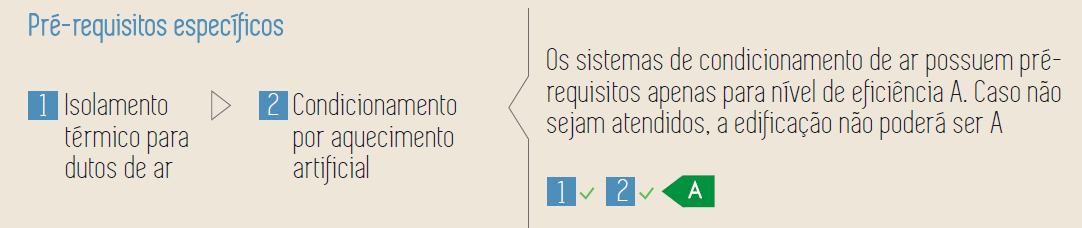
\includegraphics[width = 1.1\textwidth]{Figuras/diagrama_ar.PNG}
\caption{Pré-requisitos específicos para o sistema de condicionamento de ar.}
\label{diagrama_ar}
\textbf{Fonte:} Retirado de \cite{ManualEE}.
\end{figure}

\subsection{Isolamento térmico para dutos de ar}

Nos sistemas de aquecimento e de refrigeração, o isolamento das tubulações devem ter uma espessura mínima, na qual, as especificações devem ser consultada no RTQ-C, isso é recomendado também para projetos de edificações, onde é necessário adotar um sistema de aquecimento artificial.\cite{ManualEE}

\subsection{Condicionamento por aquecimento artificial}

Existem parâmetros mínimos de eficiência energética, que medem a relação entre a quantidade de calor fornecido ao ambiente e a energia consumida nos  sistemas com bomba de calor, aquecedores de acumulação a gás e sistemas unitários de condicionamento de ar com ciclo reverso. No RTQ-C, está previsto as especificações permitidas, e portanto, deve ser consultado. Essas exigências são para os projetos de edifícios, onde se faz necessário implementar um sistema de aquecimento artificial.\cite{ManualEE}

\end{comment}

\begin{comment}



\section{Sistema de Iluminação}

O Ministério do Meio Ambiente, no documento ``EFICIÊNCIA ENERGÉTICA: GUIA PARA ETIQUETAGEM DE EDIFÍCIOS''\cite{ManualEE}, diz:

\begin{quotation}
``A luz natural está disponível
na maior parte das horas
do dia, mas não vem sendo
explorada adequadamente
pela maioria dos projetos. O
seu uso correto e eficiente
deveria ser estimulado de
forma combinada com a
iluminação artificial, essencial
para permitir o trabalho em
locais distantes da fachada
e em horários em que a luz
natural não atinge os níveis
de iluminação mínimos
adequados.''\cite{ManualEE}
\end{quotation}

De fato, a luz natural poderia ser melhor utilizada, como alternativa, tanto para geração de energia elétrica, utilizando sistemas fotovoltaicos, bem como, na questão da iluminação zenital, diminuindo assim, a necessidade da iluminação artificial, a qual tem sido a opção dos projetos de edificações.

Como nos projetos de edificações, principalmente as públicas, comerciais e de serviços, a iluminação artificial tem sido a principal escolha, vê-se necessário considerar níveis corretos de luminosidade, que por sua vez, devem ser capazes de diminuir os consumo de energia e de carga térmica.\cite{ManualEE}

Para a obtenção da ENCE parcial do sistema de iluminação, deve-se levar em consideração três pré-requisitos específicos, que são: Divisão dos
circuitos, Contribuição da luz natural e Desligamento automático do sistema de iluminação. O nível da etiqueta a ser obtida será conforma mostra a Figura \ref{diagrama_iluminacao}.

\begin{figure}[H]
\centering
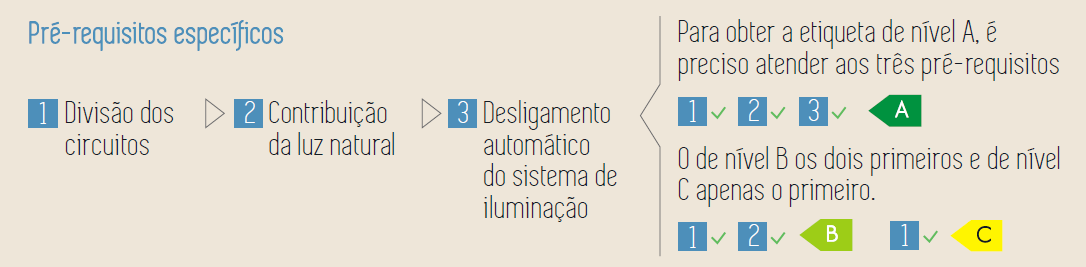
\includegraphics[width = 1.1\textwidth]{Figuras/diagrama_iluminacao.PNG}
\caption{Pré-requisitos específicos para o sistema de iluminação.}
\label{diagrama_iluminacao}
\textbf{Fonte:} Retirado de \cite{ManualEE}.
\end{figure}

\subsection{Divisão dos circuitos}

No RTQ-C, está previsto que cada ambiente fechado por paredes, ou divisórias, até o teto, deve conter no mínimo um dispositivo de controle manual para o acionamento independente da iluminação interna do ambiente, e esse controle manual, deve ser de fácil acesso e localizado de forma que possa ver todo o sistema de iluminação que está sendo controlado. Não sendo possível a visualização de todo o ambiente iluminado, é necessário apresentar ao usuário, uma representação gráfica do ambiente, especificando qual a área abrangida pelo controle manual. Por questões de segurança, ambientes de uso público poderão ter o controle manual em local de acesso a funcionários.\cite{RTQ-C}

O RTQ-C prevê também que para áreas superiores à 250 m$^2$, cada dispositivo de controle instalado, deve controlar: 
\begin{itemize}
\item Uma área de até 250 m$^2$ para ambientes com até 1000 m$^2$;
\item Uma área de até 1000 m$^2$ para ambientes maiores do que 1000 m$^2$.
\end{itemize}

A Figura \ref{iluminacao1}, mostra um exemplo de divisão de circuitos, nota-se que para uma área de 600 m$^2$, tem-se que um dispositivo de controle manual, controla os primeiros 250 m$^2$, e o outro dispositivo, controla mais 250 m$^2$, como previsto no RTQ-C.

\begin{figure}[H]
\centering
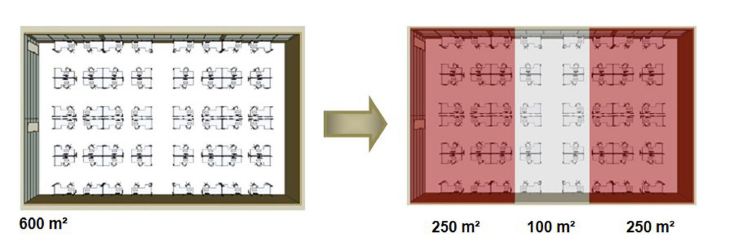
\includegraphics[width = 1.1\textwidth]{Figuras/iluminacao1.PNG}
\caption{Exemplo de divisão de circuitos para um ambiente com área superior a 250 m$^2$.}
\label{iluminacao1}
\textbf{Fonte:} Retirado de \cite{ManualEE}.
\end{figure}

\subsection{Contribuição da luz natural}

Como prevê o RTQ-C, os critérios para a contribuição da luz natural:

\begin{quotation}
``Ambientes com abertura(s) voltada(s) para o ambiente externo ou para átrio não coberto
ou de cobertura translúcida e que contenham mais de uma fileira de luminárias paralelas
à(s) abertura(s) devem possuir um controle instalado, manual ou automático, para o
acionamento independente da fileira de luminárias mais próxima à abertura, de forma a
propiciar o aproveitamento da luz natural disponível. Unidades de edifícios de meios de
hospedagem são exceção a este pré-requisito.''\cite{RTQ-C}
\end{quotation}

Algumas questões são essenciais para se obter um nível elevado de eficiência, quando se diz respeito à contribuição da luz natural. Como por exemplo, O projeto da edificação possui um sistema que considera a contribuição da luz natural na iluminação do ambiente? As luminárias dispostas próximas as janelas contém um dispositivo de desligamento independente do restante do sistema?\cite{ManualEE}

Ao realizar o projeto da edificação, deve-se atentar a essas questões, e tentar solucioná-las, uma vez que, ao serem consideradas no projeto, acarretará em uma diminuição do consumo de energia elétrica do edifício, obtendo assim, um bom nível de eficiência energética.

\subsection{Desligamento automático do sistema de iluminação}

No RTQ-C, é previsto que, o sistema de iluminação, de ambientes com áreas superiores a 250 m$^2$, deve conter um dispositivo de controle automático para o desligamento da iluminação, e este dispositivo deve operar de acordo com uma das seguintes opções:\cite{RTQ-C}

\begin{itemize}
\item Um sistema automático com desligamento da iluminação em um horário pré-determinado. Deverá existir uma programação independente para um limite de área de até 2500 m$^2$;
\item Um sensor de presença que desligue a iluminação 30 minutos após a saída de todos ocupantes;
\item Um sinal de um outro controle ou sistema de alarme que indique que a área está desocupada.\cite{RTQ-C}
\end{itemize}


Existem algumas exceções para o critério de desligamento automático do sistema de iluminação, os quais são:

\begin{itemize}
\item Ambientes que devem propositadamente funcionar durante 24 h;
\item Ambientes onde existe tratamento ou repouso de pacientes;
\item Ambientes onde o desligamento automático da iluminação pode comprovadamente oferecer riscos à integridade física dos usuários.\cite{RTQ-C}
\end{itemize}

\subsection{Procedimento de determinação da eficiência}

O intuito de realizar esse procedimento é estabelecer o limite de potência de iluminação para os ambientes internos da edificação. Os níveis de eficiência energética para o sistema de iluminação para a obtenção da ENCE parcial variam de A até E, sendo A o mais eficiente, e consequentemente, E o menos eficiente. Vale ressaltar que o sistema de iluminação corresponde a 30\% da pontuação total da eficiência energética da edificação.\cite{RTQ-C}

Existem dois métodos de avaliação do sistema de iluminação, os quais são: Método da área do edifício e método das atividades do edifício. Para a obtenção da ENCE parcial, deve-se escolher um desses dois métodos.

Conforme mostra o RTQ-C, há alguma exceções que não devem ser consideradas no cálculo da potência instalada da iluminação, os sistemas que forem complementares à iluminação geral e com controle independente, não serão considerados, nas seguintes situações:\cite{RTQ-C}

\begin{itemize}
\item Iluminação de destaque que seja parte essencial para o funcionamento de galerias, museus e monumentos;
\item Iluminação contida ou parte integrante de equipamentos ou instrumentos, desde que instalada pelo próprio fabricante, como lâmpadas de refrigeradores, geladeiras, etc;
\item Iluminação especificamente projetada para uso exclusivo em procedimentos médicos ou dentários e iluminação contida em equipamentos médicos ou
dentários;
\item Iluminação contida em refrigeradores e \textit{freezers}, tanto abertos quanto fechados por vidro; 
\item Iluminação totalmente voltada a aquecimento de alimentos e em equipamentos de preparação de alimentos;
\item Iluminação totalmente voltada ao crescimento de plantas ou sua manutenção;
\item Iluminação em ambientes especificamente projetados para uso de deficientes visuais;
\item Iluminação em vitrines de lojas varejistas, desde que a área da vitrine seja fechada por divisórias cuja altura alcance o forro;
\item Iluminação em ambientes internos que sejam especificamente designados como um bem cultural tombado, de acordo com o IPHAN – Instituto do Patrimônio Histórico Artístico Nacional ou outros órgãos municipais ou estaduais de competência análoga;
\item Iluminação totalmente voltada à propaganda ou à sinalização;
\item Sinais indicando saída e luzes de emergência;
\item Iluminação à venda ou sistemas de iluminação para demonstração com propósitos educacionais;
\item Iluminação para fins teatrais, incluindo apresentações ao vivo e produções de filmes e vídeos;
\item Áreas de jogos ou atletismo com estrutura permanente para transmissão pela televisão;
\item Iluminação de circulação externa;
\item Iluminação de tarefa ligada diretamente em tomadas, como luminária de mesa.\cite{RTQ-C}
\end{itemize}

\subsubsection{Método da área do edifício}

O método da área do edifício tem como intuito, a avaliação conjunta de todos os ambientes da edificação, atribuindo um valor único para o limite da potência de iluminação, este método deve ser utilizado, em edificações que possuem até três atividades principais, ou que possuem atividades que ocupem mais de 30\% da área da edificação.\cite{RTQ-C}

Primeiramente, com base na Tabela \ref{tab1}, deve-se identificar a atividade principal da edificação, bem como, a densidade de potência de iluminação limite($DPI_L$), medida em $W/m^2$, para cada nível de eficiência. Vale a pena ressaltar que para edificações com atividades não-listadas deve-se adotar uma atividade similar.\cite{RTQ-C}



\begin{table}[H]
  \centering
  \caption{Limite máximo aceitável de densidade de potência de iluminação ($DPI_L$) para o nível de eficiência pretendido – Método da área do edifício.}
    \begin{tabular}{ccccc}
    \hline
    Função do Edifício & \begin{tabular}[c]{@{}l@{}}Densidade de\\Potência \\de Iluminação  \\limite ($W/m^2$)\\ (Nível A) \end{tabular} &  \begin{tabular}[c]{@{}l@{}}Densidade de\\Potência \\de Iluminação  \\limite ($W/m^2$) \\(Nível B) \end{tabular} &  \begin{tabular}[c]{@{}l@{}}Densidade de\\Potência \\de Iluminação  \\limite ($W/m^2$) \\(Nível C) \end{tabular} &  \begin{tabular}[c]{@{}l@{}}Densidade de\\Potência \\de Iluminação  \\limite ($W/m^2$)\\ (Nível D) \end{tabular} \\    \hline
Academia & 9,5 & 10,9 & 12,4 & 13,8 \\
Armazém & 7,1& 8,2& 9,2& 10,3  \\
Biblioteca &12,7& 14,6& 16,5& 18,4   \\
Bombeiros &7,6 &8,7 &9,9 &11,0                 \\
Centro de Convenções &11,6& 13,3 &15,1& 16,8     \\
Cinema &8,9 &10,2& 11,6& 12,9                    \\
Comércio &15,1 &17,4 &19,6 &21,9                 \\
Correios& 9,4& 10,8& 12,2& 13,6                 \\
Venda e Locação de Veículos &  8,8 &10,1 &11,4 &12,8   \\                  

Escola/Universidade &10,7 &12,3 &13,9& 15,5      \\
Escritório &9,7 &11,2 &12,6 &14,1               \\
Estádio de esportes &8,4 &9,7& 10,9& 12,2        \\
Garagem – Ed. Garagem &2,7& 3,1 &3,5& 3,9       \\
Ginásio &10,8 &12,4& 14,0& 15,7                  \\
Hospedagem, Dormitório &6,6 &7,6 &8,6& 9,6       \\
Hospital &13,0& 15,0& 16,9& 18,9                \\
Hotel &10,8 &12,4 &14,0 &15,7                   \\
Igreja/Templo &11,3 & 13,0 &14,7& 16,4          \\
Restaurante &9,6 &11,0 &12,5 &13,9              \\
Restaurante: Bar/Lazer &10,7& 12,3& 13,9& 15,5   \\
Restaurante: Fast-food &9,7 &11,2 &12,6 &14,1    \\
Museu &11,4& 13,1 &14,8 &16,5                   \\
Oficina &12,9 &14,8 &16,8 &18,7                  \\
Penitenciária &10,4 &12,0 &13,5 &15,1            \\
Posto de Saúde/Clínica &9,4& 10,8& 12,2& 13,6    \\
Posto Policial &10,3 &11,8 &13,4& 14,9          \\
Prefeitura – Inst. Gov. &9,9 &11,4 &12,9 &14,4  \\
Teatro &15,0 &17,3& 19,5& 21,8                   \\
Transportes &8,3 &9,5 &10,8 &12,0               \\
Tribunal& 11,3 &13,0& 14,7& 16,4    \\\hline  
    \end{tabular}%
  \label{tab1}
   \textbf{Fonte:} Retirado de \cite{RTQ-C}.
\end{table}%

O segundo passo desse método, é determinar a área da edificação, e então, multiplica-se o valor encontrado para a área pelo valor da $DPI_L$, mostrado na Tabela \ref{tab1}, para encontrar a potência limite da edificação. Se a edificação possuir três atividades principais, deve-se determinar a $DPI_L$ para cada atividade, e também a área iluminada de cada atividade. A potência limite total da edificação, será a soma das potências limites de cada uma das atividades principais da edificação. Vale ressaltar que, o nível de eficiência energética será feita com base na potência total instalada na edificação, e não por atividade principal.\cite{RTQ-C}

Com os valores das potências limites obtidos, deve-se compará-los com o valor de potência total instalada na edificação, para poder determinar o nível de eficiência energética do edifício. Após a determinação do nível de eficiência, deve-se verificar se cada ambiente atende aos pré-requisitos específicos do sistema de iluminação descritos anteriormente.\cite{RTQ-C}

Caso algum dos ambientes não atenda à algum dos pré-requisitos, o valor do EqNumDPI deve ser alterado, com base na ponderação entre os níveis de eficiência e potência instalada dos ambientes que não atenderam aos pré-requisitos e a potência instalada e o nível de eficiência encontrado para o sistema de iluminação.\cite{RTQ-C}

\subsubsection{Método das atividades do edifício}

O método das atividades do edifício, tem como objetivo, avaliar separadamente os ambientes da edificação, e deve ser utilizado em edificações nas quais o método da área do edifício não se aplica.\cite{RTQ-C}

Primeiramente, com base na Tabela mostrada nas Figuras \ref{tab2_1}, \ref{tab2_2} e \ref{tab2_3}, deve-se identificar as atividades encontradas na edificação, e consultar a $DPI_L$ limite para cada nível de eficiência energética de cada uma das atividades. Vale a pena ressaltar que para edificações com atividades não-listadas deve-se adotar uma atividade similar.\cite{RTQ-C}

Para obter o valor da potência limite para cada atividade, deve-se multiplicar o valor da área iluminada de cada atividade, pela $DPI_L$. Analogamente ao método da área do edifício, a potência limite para o edifício será a soma das potências limites das atividades.\cite{RTQ-C}

Com o valor da potência limite do edifício calculada, deve-se calcular a potência instalada, e compará-las, para obter o valor do EqNumDPI do sistema de iluminação.

Caso algum dos ambientes não atenda à algum dos pré-requisitos, o valor do EqNumDPI deve ser alterado, com base na ponderação entre os níveis de eficiência e potência instalada dos ambientes que não atenderam aos pré-requisitos e a potência instalada e o nível de eficiência encontrado para o sistema de iluminação.\cite{RTQ-C}

\section{Dimerização}

Define-se dimerização, com sendo o controle da intensidade de luz, ou seja,  ao se instalar lâmpadas que são dimerizáveis, essas, são capazes de regular a intensidade do brilho emitido pela lâmpada, de forma a controlar a iluminação visual de um ambiente da edificação.\cite{Dimer}

As lâmpadas incandescentes, que por muito tempo foram as mais utilizadas, eram lâmpadas dimerizáveis, uma vez que podia-se regular a intensidade de seu brilho, porém, como essas lâmpadas possuem um elevado consumo de energia elétrica, e com a chegada das lâmpadas de LED, que são mais econômicas, fomentou em um afastamento por muito tempo da dimereização.  No entanto, já se é possível realizar a dimerização nas lâmpadas de LED, que são de baixo consumo.\cite{Dimer}

O dimmer, é o aparelho que realiza a dimerização, ele é responsável por controlar a intensidade da luz de uma certa lâmpada, a qual, ilumina um ambiente de uma edificação.  Este dispositivo, substitui o interruptor, uma vez que, o interruptor serve apenas para ligar e desligar a lâmpada, o dimer permite que o usuário, deslize seu botão, permitindo-o deixar a intensidade da luz do ambiente, como desejar .\cite{Dimer}

Dentre todas as funções do dimmer, ele também é responsável por aumentar o tempo de vida útil da lâmpada, uma vez que,  ele diminui a tensão aplicada na lâmpada, para poder obter a intensidade da luz desejada. O dimmer, é capaz de garantir um melhor conforto para a visão do usuário. \cite{Dimer}

Existem dois tipos de dimmer, o dimmer eletrônico, o qual, ajuda na economia da energia, uma vez que corta a onda senoidal da tensão, o que reduz o consumo. Existe também o dimmer resistivo, o qual consome a diferença de energia, que iria para a lâmpada, reduzindo assim o brilho. Os dois tipos de dimmer, aumentam a vida útil das lampadas,  que têm a tensão aumentada de forma suave, diferentemente do interruptor, que aplica a tensão máxima na lâmpada. \cite{Dimer2}

Há vários motivos, que levam a utilização da dimerização no sistema de iluminação de um ambiente. Além das características já citadas,  o dimmer não necessidade de uma grande demanda de manutenção no sistema de iluminação, e principalmente, ao instalar um sistema de dimerização, há uma diminuição significativa no consumo de energia elétrica .\cite{Dimer}

A dimerização, pode ser utilizada para aproveitar a luz natural de forma inteligente, vinculado com o uso da lâmpada de LED, que possui um baixo consumo, equilibrando a intensidade da luz da lâmpada com a luz natural que entra no ambiente,  acarretará em uma grande diminuição do consumo de energia elétrica, e consequentemente, uma diminuição nos gastos com energia.

\section{Tipos de Lâmpadas}

Segundo a Copel, existem atualmente onze tipos de lâmpadas no mercado, as quais são: Incandescentes, Fluorescentes, Halógenas, Dicróicas, Vapor de mercúrio, De Sódio(baixa pressão), De Sódio(alta pressão), Mista, Fluorescentes compactas, Multi-vapores metálicos e LED.\cite{Copel}

\subsection{Lâmpadas Incandescentes}

As lâmpadas incandescentes, são as mais encontradas nas edificações, elas emitem luz a partir de um filamento incandescente, ou seja, a corrente elétrica passa por um filamento, que aquece, e assim, emite uma luz visível. Esse tipo de lâmpada possui uma eficiência luminosa muito baixa, cerca de 12 lm/W. Possuem um baixo custo, porém, seu tempo de vida útil também é baixo, cerca de 1000 h. A Figura \ref{lamp_inc}, mostra como é uma lâmpada incandescente.\cite{Copel}


\begin{figure}[H]
\centering
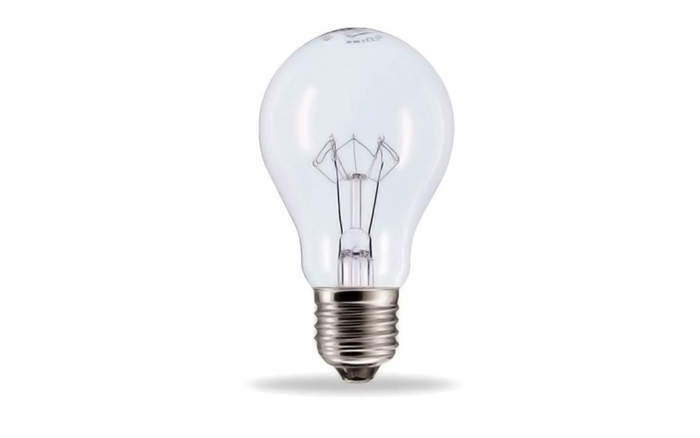
\includegraphics[width = 1.1\textwidth]{Figuras/lamp_inc.jpg}
\caption{Exemplo de Lâmpada Incandescente.}
\label{lamp_inc}
\textbf{Fonte:} Retirado de \cite{Figlamp1}.
\end{figure}

Em ambientes grandes, com frequência permanente, deve-se tomar cuidado ao utilizar esse tipo de lâmpada, uma vez que, possuem um alto consumo de energia, elas também podem elevar a carga térmica, o que gera um maior gasto com condicionadores de ar. Este tipo de lâmpada pode ser adaptada com um sistema de dimerização, já descrito anteriormente.\cite{Copel}


Existe um nível mínimo de eficiência energética, que deve ser obedecido pelas lâmpadas incandescentes, que foi estabelecido através da da Portaria Interministerial 1.007, de 31/12/2010, que proíbe a comercialização de lâmpadas incandescentes com potência superior a 60W.\cite{Copel}

\subsection{Lâmpadas Fluorescentes}

As lâmpadas fluorescentes, funcionam através de um gás, que quando ionizado, emite radiação ultravioleta, e essa radiação, ao incidir sobre uma camada fluorescente na superfícies dos tubos de vidro, acaba se transformando em luz visível. Para o funcionamento desse tipo de lâmpada, faz-se necessário o uso de um reator, os quais podem ser externos ou integrados. Ao se comparar com a lâmpada incandescente, as lâmpadas fluorescentes possuem um maior tempo de vida útil, por volta de 7500 h, e a sua eficiência luminosa superam os 70 lm/W, cerca de cinco vezes maior que a eficiência luminosa das lâmpadas incandescentes. A Figura \ref{lamp_flu}, mostra como é uma lâmpada fluorescente.\cite{Copel}



\begin{figure}[H]
\centering
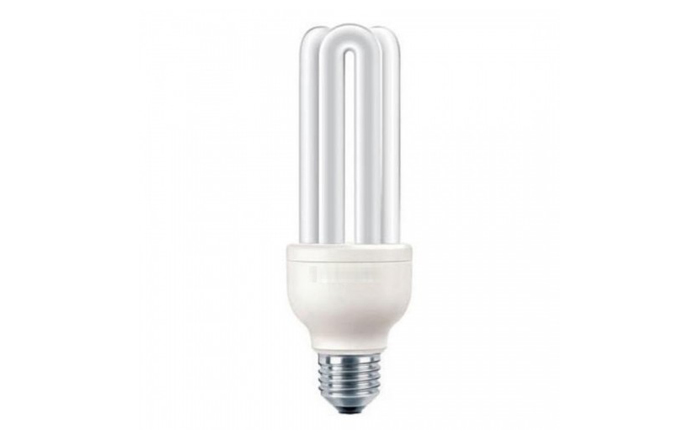
\includegraphics[width = 1.1\textwidth]{Figuras/lamp_flu.jpg}
\caption{Exemplo de Lâmpada Fluorescente.}
\label{lamp_flu}
\textbf{Fonte:} Retirado de \cite{Figlamp1}.
\end{figure}

As lâmpadas fluorescentes compactas, funcionam igual as normais, elas possuem uma eficiência luminosa entre 50 e 70 lm/W e representam uma economia de energia, em relação às lâmpadas incandescentes, em torno de 75\% a 80\%, e não são dimerizáveis. A Figura \ref{lamp_flucomp}, mostra como é uma lâmpada fluorescente compacta.\cite{Copel}



\begin{figure}[H]
\centering
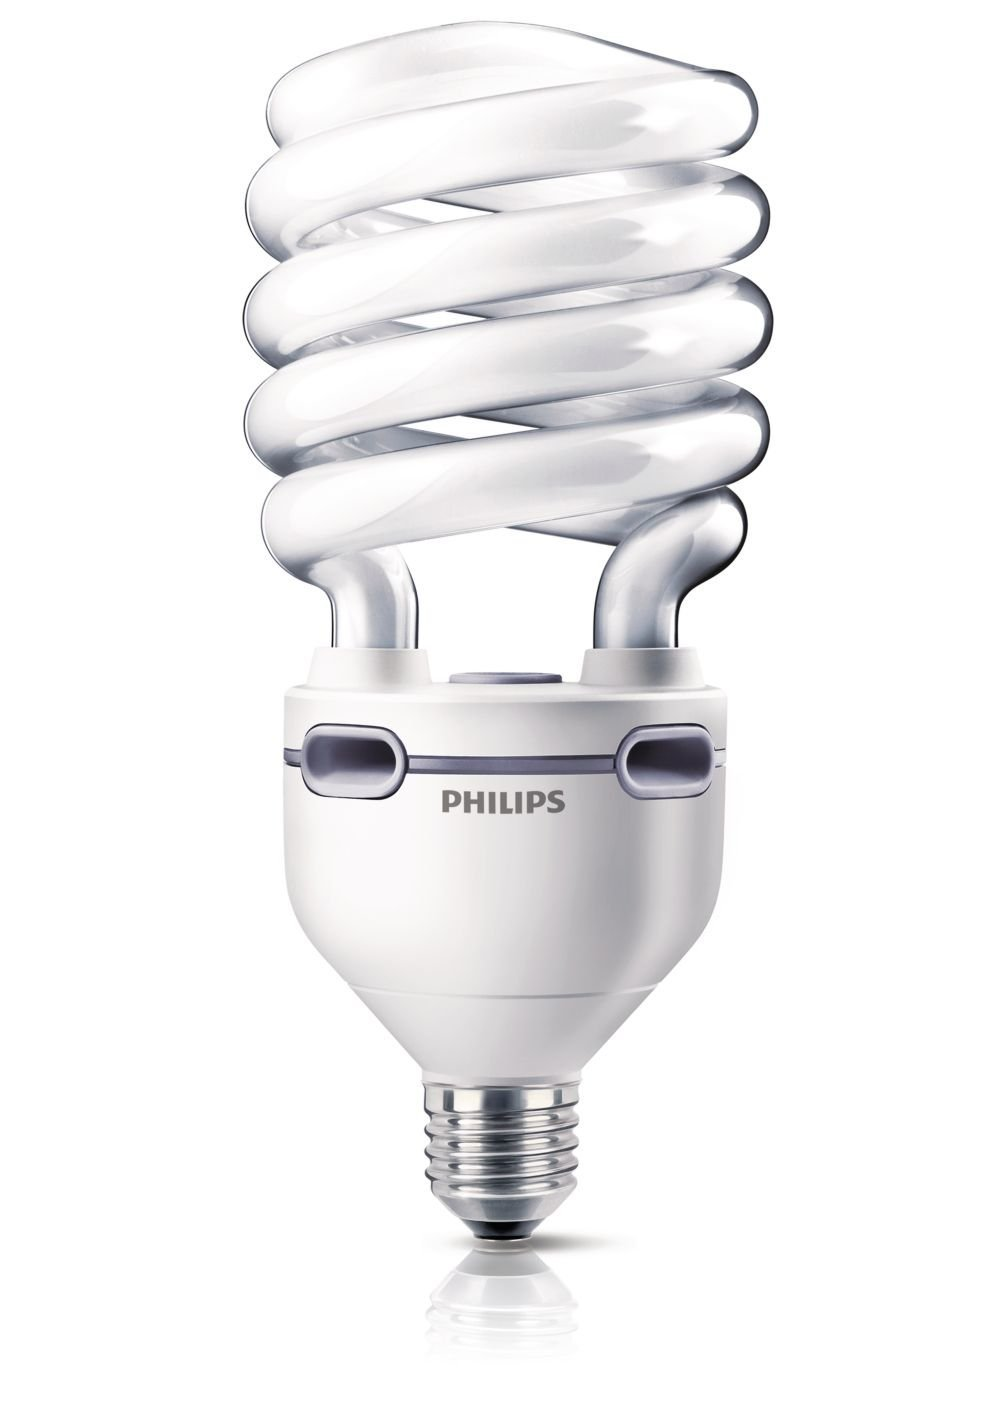
\includegraphics[width = 0.5\textwidth]{Figuras/lamp_flucomp.jpg}
\caption{Exemplo de Lâmpada Fluorescente Compacta.}
\label{lamp_flucomp}
\textbf{Fonte:} Retirado de \cite{Figlamp1}.
\end{figure}

\subsection{Lâmpadas Halógenas}

As lâmpadas halógenas possuem um funcionamento similar ao das lâmpadas incandescentes, porém, com uma redução no consumo de energia, em torno de 25\% a 40\%, elas são compactas e possuem uma vida útil de 2000 h. Esse tipo de lâmpada permite a implementação de um sistema de dimerização. A Figura \ref{lamp_halo}, mostra como é uma lâmpada halógena.\cite{Copel}


\begin{figure}[H]
\centering
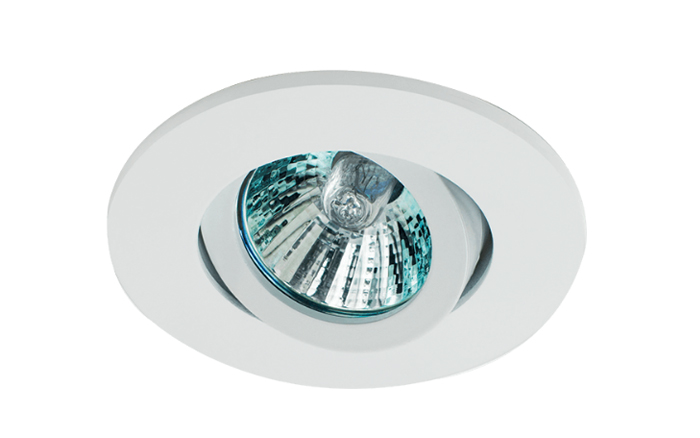
\includegraphics[width = 1.1\textwidth]{Figuras/lamp_halo.jpg}
\caption{Exemplo de Lâmpada Halógena.}
\label{lamp_halo}
\textbf{Fonte:} Retirado de \cite{Figlamp1}.
\end{figure}


\subsection{Lâmpadas de LED}

As lâmpadas de LED, são as mais econômicas existentes no mercado, seu funcionamento consiste em, um material semicondutor, que ao ser energizado, emite uma luz visível. Os modelos comerciais, atingem uma eficiência luminosa entre 80 e 100 lm/W. Elas possuem uma vida útil superior a 1500 h, podendo variar conforme o fabricante. A Figura \ref{lamp_led}, mostra como é uma lâmpada de LED.\cite{Copel}


\begin{figure}[H]
\centering
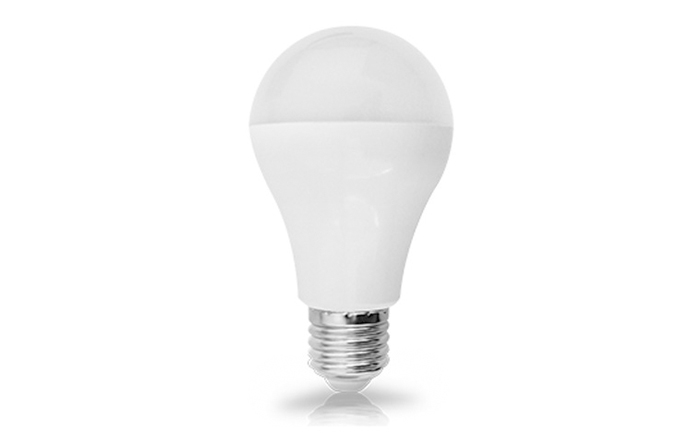
\includegraphics[width = 1.1\textwidth]{Figuras/lamp_led.jpg}
\caption{Exemplo de Lâmpada de LED.}
\label{lamp_led}
\textbf{Fonte:} Retirado de \cite{Figlamp1}.
\end{figure}


As lâmpadas de LED, possui um valor elevado se comparada às lâmpadas incandescentes, porém, o investimento é compensado à longo prazo, uma vez que uma lâmpada de LED consegue de apenas 10W é equivalente à uma lâmpada incandescente de 60W, ou seja, o consumo de energia de uma lâmpada de LED, é significantemente inferior, ao consumo de energia de uma lâmpada incandescente, o que resulta em uma grande redução no custo da energia elétrica.

\end{comment}
































































				  % Capítulo 2 - Texto do cap2.tex
%%
\chapter{Desenvolvimento}\label{chp:desenvol}
\vspace{-1.5cm}
\noindent\rule{\columnwidth}{1.2mm}



\section{Metodologia}

A metodologia do se divide entre, reconhecimento do projeto, execução e aprimoramento das etapas, tudo atrelado as normativas.

A primeira etapa é reconhecer o projeto em si, tendo em vista a planta estrutural e construindo um diagrama de fluxo de toda a parte elétrica do sistema, transpondo todo o trecho que o grão deve passar, desde sua chegada até a saída do complexo. Conhecendo o fluxo desejado de grãos e a capacidade de armazenamento é possível realizar o dimensionamento das potências dos motores de cada etapa. 

A divisão dos motores pode ser realizada a a partir da aplicação de cada motor, ou da área em que ele esta sendo utilizado:
Dentre as aplicações tem-se:

\begin{itemize}
    \item Elevadores
    \item Secadores
    \item Aeração
    \item Transportadores
\end{itemize}

Toda  a distribuição dos circuitos é realizada a partir do quadro de centro de controle de máquinas (CCM), é nele que fica todo o sistema de proteção e de partida de cada motor. Assim, tudo permanece de forma centralizada, facilitando a operação, manutenção, controle a aplicabilidade do sistema.

\subsection{Organização}


\subsection{Dimensionamento Cabos Elétricos}

Para o dimensionamento de cabos elétricos de baixa tensão, é essencial utilizar como base  a norma NBR 5410. Devem ser dimensionados os condutores de fase, neutro (para os casos onde existem) e os condutores de aterramento. %cite

\subsubsection{Condutores}

Para dimensionamento dos condutores de fase, são levados em conta alguns critérios: 
O critério de capacidade de condução de corrente dos cabos elétricos, tem como objetivo proteger os cabos dos efeitos térmicos causados pela condução de corrente, onde a corrente  que é transportada pelo cabo incluindo as harmônicas, não deve elevar a temperatura máxima além do permitido para o cabo em uso. 

A norma fornece tabelas de consulta, onde pode ser visto a máxima corrente suportada para as funções normais de trabalho para cada respectiva bitola, de acordo com o método de instalação utilizado. Sendo sendo duas tabelas, para cabos cuja temperatura máxima suportada é de 70 $^{\circ}$c e para cabos cuja temperatura máxima suportada é de 90 $^{\circ}$c. Os cabos com grau maior de proteção suportam maiores corrente de trabalho, porém possuem um maior custo. 

Para exemplificar analisamos um cabo de $6mm^2$, com 3 condutores e  método de instalação D (cabo multipolar em eletroduto enterrado no solo), o cabo com isolação PVC e temperatura no condutor de  70 $^{\circ}$c tem uma capacidade de condução de corrente de 39 A, já o cabo com isolação e EPR ou XLPE e temperatura no condutor de  90 $^{\circ}$c tem uma capacidade de corrente de 46A 

Como a maior parte dos circuitos deste projeto é de motores elétricos é adotado para utilização  os cabos de 90 $^{\circ}$c de proteção.

\subsection{Fatores de correção}
A corrente nominal do motor é indicada na plaqueta e também pode ser obtida partir da potência do motor e da tensão de trabalho. Porém, para dimensionamento dos cabos alguns fatores de correção devem ser aplicados, a fim de garantir que o dimensionamento seja adequado para cada caso específico de utilização. 

Cada fator de correção trará um valor diferente de corrente, para o o dimensionamento do cabo, deve ser utilizado o valor de maior corrente, ou seja, o pior caso.

\subsubsection{Fator de temperatura ambiente}

\subsubsection{Fator de agrupamento}
O fator de agrupamento leva em conta os outros circuitos e cabos que são levados juntamente com 

\subsection{Tubulação}


\subsection{Iluminação}			  % Capítulo 3 - Texto do cap3.tex
%%
\chapter{Resultados}\label{chp:resultados}
\vspace{-1.5cm}
\noindent\rule{\columnwidth}{1.2mm}
\vspace{0.1cm}

\section{Resultados Obtidos}

Ao aplicar o método da área do edifício, obteve-se os valores da densidade de potência de iluminação limite para cada nível energético, da edificação estudada, com base nas especificações do RTQ-C, para a atividade principal Escola/Universidade, da Tabela \ref{tab1}. Vale ressaltar que a edificação possui uma área total de 5892,12 $m^2$, multiplicando-a pelos coeficientes da Tabela \ref{tab1}, encontrou-se os valores mostrados na Tabela \ref{tab_dpil}.

\begin{table}[H]
\centering
\caption{Valores das potências limites para cada nível, da edificação estudada.}
\label{tab_dpil}
\begin{tabular}{ll}\hline
Nível Energético & Potência (W) \\\hline
A                & 63045,684        \\
B                & 72473,076        \\
C                & 81900,468        \\
D                & 91327,86   \\\hline     
\end{tabular}
\end{table}

Com o trabalho realizado em campo, detectou-se certas características do sistema de iluminação da edificação analisada. Primeiramente, constatou-se que a edificação não atende ao critério de desligamento automático do sistema de iluminação, e isso já inviabiliza a obtenção da ENCE parcial de nível A para essa edificação. A edificação, em alguns ambientes, não atende ao critério da contribuição da luz natural em sua totalidade, uma vez que observou-se que em algumas salas, as janelas possuem películas de controle solar, que dificulta a entrada a luz natural no ambiente, e também, em certos ambientes, a fileira de luminárias próximas à janela, não possuem um controle para acionamento independente, que faz com que as lâmpadas fiquem acesas mesmo com a entrada da luz natural no ambiente, e esse fator, combinado com o não atendimento do critério de desligamento automático do sistema de iluminação, inviabiliza que a edificação receba uma ENCE parcial de nível A e de nível B para o sistema de iluminação.

Porém, a edificação apresentou alguns aspectos positivos, constatou-se que em todos os ambientes, o critério da divisão de circuitos é atendido. Observou-se também que algumas medidas para a redução do consumo energético foram tomadas, em uma ala do segundo pavimento da edificação, as lâmpadas utilizadas são de LED com potência de 18 W, com luminárias que utilizam 2 lâmpadas apenas, e em grande parte do edifício, as lâmpadas instaladas, são fluorescentes de 32 W, com luminárias que utilizam apenas 2 lâmpadas.

Vale ressaltar que, a edificação passou por uma reforma, e possui alguns ambientes, que ainda utilizam lâmpadas incandescentes de 40 W, com luminárias que utilizam 4 lâmpadas. Os ambientes construídos na reforma, são os que apresentam as medidas de redução de consumo energético descrito anteriormente.

Para medir o valor da potência total instalada, realizou-se uma contagem do número de lâmpadas utilizadas em cada ambiente da edificação, levando em consideração o tipo de lâmpada e a potência de cada lâmpada instalada. As Tabelas \ref{tab_terreo}, \ref{tab_pav1} e \ref{tab_pav2}, mostram os valores das potências instaladas de cada ambiente dos pavimentos do edifício, bem como o valor total da potência instalada em cada pavimento. Os ambientes descritos são mostrados nas plantas do edifício, que são mostradas nas Figuras \ref{pav_terreo}, \ref{pav2} e \ref{pav3}, que representam os pavimentos térreo, segundo pavimento e terceiro pavimento, respectivamente. 



\begin{table}[H]
\centering
\caption{Potência instalada do Pavimento Térreo.}
\label{tab_terreo}
\begin{tabular}{ll}\hline
Ambiente                   & Potência(W) \\\hline
Sala 1021                  & 384         \\
Sala 1022                  & 384         \\
Sala 1023                  & 384         \\
Sala 1024                  & 384         \\
Sala 1025                  & 384         \\
Sala 1026                  & 384         \\
Sala 1027                  & 384         \\
Corredor1                  & 1408        \\
Hall                       & 448         \\
Copa                       & 320         \\
Almoxarifado Tec. Elétrica & 160         \\
Sala 1001                  & 1280        \\
Sala 1002                  & 1280        \\
Sala 1003                  & 1280        \\
Sala 1004                  & 1280        \\
Sala 1005                  & 1280        \\
Corredor2                  & 1600        \\
Sala 1006/1007             & 1920        \\
Sala 1008                  & 960         \\
Sala 1009/1010             & 1920        \\
Banheiro Masc.             & 240         \\
Banheiro Fem.              & 160         \\
Escada                     & 160         \\\hline
Total                      & 18384  \\\hline    
\end{tabular}
\end{table}

\begin{table}[H]
\centering
\caption{Potência instalada do Segundo Pavimento.}
\label{tab_pav1}
\begin{tabular}{ll}\hline
Ambiente       & Potencia (W) \\\hline
Sala 1011      & 1280         \\
Sala 1012      & 1280         \\
Sala 1013      & 1280         \\
Sala 1014      & 1280         \\
Sala 1015/1016 & 2560         \\
Sala 1017      & 1280         \\
Sala 1018      & 1280         \\
Sala 1019      & 1280         \\
Sala 1020      & 1280         \\
Corredor 3     & 1440         \\
Hall           & 384          \\
Sala MM1       & 324          \\
Sala MM2       & 324          \\
Sala MM3       & 324          \\
Sala MM4       & 324          \\
Sala MM5       & 324          \\
Secret. TRU    & 144          \\
Secret. CIV    & 144          \\
Secret. GERAL  & 360          \\
Secret. ELE    & 144          \\
Secret. ARQ    & 144          \\
Colegiado      & 108          \\
Lig 1          & 324          \\
Lig 2          & 324          \\
Informática    & 144          \\
L.A.U          & 324          \\
Banheiro Masc. & 240          \\
Banheiro Fem.  & 240          \\
Escada         & 160          \\
Corredor 4     & 540          \\
Almoxarifado   & 80           \\\hline
Total          & 19664  \\\hline       
\end{tabular}
\end{table}


\begin{longtable}[H]{ll}
\caption{Potência instalada do Terceiro Pavimento.}
\label{tab_pav2}\\\hline
Ambiente & Potencia (w) \\\hline
\endfirsthead
%
\endhead
%
Sala MM 6 & 576 \\
Sala MM 7 & 576 \\
Sala MM 8 & 576 \\
Sala MM 9 & 576 \\
Sala MM 10 & 576 \\
Sala MM 11 & 576 \\
Secret. Pós-Grad. & 192 \\
Ambiente & Potencia (w) \\\hline
Acervo Pós-Grad. & 192 \\
Pós-Grad & 384 \\
Pós-Grad & 384 \\
Lab. Doc. & 192 \\
NEPEA & 1024 \\
Corredor 5 & 1152 \\
Hall & 400 \\
Copa & 320 \\
Corredor 6 & 1344 \\
Docente ELE 1 & 256 \\
Docente ELE 2 & 256 \\
Docente ELE 3 & 256 \\
Docente ELE 4 & 256 \\
Docente ELE 5 & 256 \\
Docente ELE 6 & 256 \\
Docente ELE 7 & 256 \\
Docente ELE 8 & 256 \\
Docente ELE 9 & 256 \\
Docente CIV 1 & 256 \\
Docente CIV 2 & 256 \\
Docente CIV 3 & 256 \\
Docente CIV 4 & 256 \\
Docente CIV 5 & 256 \\
Docente CIV 6 & 256 \\
Docente CIV 7 & 256 \\
Docente CIV 8 & 256 \\
Docente CIV 9 & 256 \\
Reuniões 1 & 512 \\
Reuniões 2 & 256 \\
Docente TRU 1 & 256 \\
Docente TRU 2 & 256 \\
Docente TRU 3 & 256 \\
Docente TRU 4 & 256 \\
Docente TRU 5 & 256 \\
Docente TRU 6 & 256 \\
Docente ARQ 1 & 256 \\
Docente ARQ 2 & 256 \\
Ambiente & Potencia (w) \\\hline
Docente ARQ 3 & 256 \\
Docente ARQ 4 & 256 \\
Docente ARQ 5 & 256 \\
Docente ARQ 6 & 256 \\
Docente ARQ 7 & 256 \\
Docente ARQ 8 & 256 \\
Docente ARQ 9 & 256 \\
Docente ARQ 10 & 256 \\
Banheiro Masc. & 240 \\
Banheiro Fem. & 240 \\
Escada & 80 \\\hline
Total: & 19072\\\hline
\end{longtable}

Com base nas Tabelas \ref{tab_terreo}, \ref{tab_pav1} e \ref{tab_pav2}, obteve-se que o valor total da potência instalada é de 59856 W, ao comparar com os valores limites obtidos, mostrados na Tabela \ref{tab_dpil}, nota-se que a edificação está apta a receber uma ENCE parcial de nível A, analisando a potência total da edificação. Porém a edificação, como foi dito anteriormente, não atende à um dos pré-requisitos previstos para o sistema de iluminação no RTQ-C, o de desligamento automático do sistema de iluminação, e atende parcialmente ao critério de luz natural. Com base nessas informações, deve-se fazer uma ponderação entre os níveis de eficiência e potência instalada dos ambientes que não atenderam aos pré-requisitos e a potência instalada e o nível de eficiência encontrado para o sistema de iluminação.

Levando em consideração que nenhum dos pavimentos atende ao critério de desligamento automático do sistema de iluminação, e que o critério de luz natural é atendido em parte do edifício, e também que a edificação atende em sua totalidade, ao critério de divisão de circuitos, a edificação teria uma ENCE parcial de nível C. No entanto, fazendo a ponderação com a potência instalada em cada pavimento, observando as Tabelas \ref{tab_dpil2} e \ref{tab_pavs}, pode-se ver que a potência instalada de nenhum dos pavimentos, ultrapassa a potência limite, para os pavimentos, do nível A, logo, pode-se dizer que a ENCE parcial final da edificação é de nível B.


\begin{table}[H]
\centering
\caption{Valores das potências limites para cada nível, por pavimentos.}
\label{tab_dpil2}
\begin{tabular}{ll}\hline
Nível Energético & Potência Limite (W) \\\hline
A                & 21015,23            \\
B                & 24157,69            \\
C                & 27300,16            \\
D                & 30442,62     \\\hline      
\end{tabular}
\end{table}


\begin{table}[H]
\centering
\caption{Valores das potências intaladas por pavimento.}
\label{tab_pavs}
\begin{tabular}{ll}\hline
Pavimento          & \begin{tabular}[c]{@{}l@{}}Potência instalada\\   (W)\end{tabular} \\\hline
Pavimento Térreo   & 18384                                                              \\
Segundo Pavimento  & 19664
                                                             \\
Terceiro Pavimento & 19520     \\\hline                                                        
\end{tabular}
\end{table}

\section{Projeções de Melhorias}

Analisando o segundo pavimento da edificação, conforme foi constatado, em uma ala do pavimento, a lâmpadas utilizadas são de LED, com potência de 18 W, e a outra ala, de mesma área, possuem lâmpadas incandescentes, com potência de 40 W. Como pode-se observar, nas Tabelas \ref{tab_40w} e \ref{tab_led}, e no gráfico da Figura \ref{graph2}, a ala que utiliza lâmpadas incandescentes, possui uma potência instalada muito maior, cerca de 66\% maior, que a ala que possui lâmpadas de LED, e consequentemente, uma menor eficiência energética. Vale a pena ressaltar que, na ala que possui lâmpadas incandescentes instalada, a potência instalada, representa cerca de 72\% da potência total do pavimento.



\begin{table}[H]
\centering
\caption{Potência instalada da ala que utiliza lâmpadas incandescentes de 40 W.}
\label{tab_40w}
\begin{tabular}{ll}\hline  
Ambiente       & Potência instalada (W) \\\hline  
Sala 1011      & 1280                   \\
Sala 1012      & 1280                   \\
Sala 1013      & 1280                   \\
Sala 1014      & 1280                   \\
Sala 1015/1016 & 2560                   \\
Sala 1017      & 1280                   \\
Sala 1018      & 1280                   \\
Sala 1019      & 1280                   \\
Sala 1020      & 1280                   \\
Corredor 3     & 1440                   \\\hline  
Total          & 14240  \\\hline                 
\end{tabular}
\end{table}

\begin{table}[H]
\centering
\caption{Potência instalada da ala que utiliza lâmpadas de LED de 18 W.}
\label{tab_led}
\begin{tabular}{ll}\hline  
Ambiente      & Potência instalada (W) \\\hline  
Sala MM1      & 324                    \\
Sala MM2      & 324                    \\
Sala MM3      & 324                    \\
Sala MM4      & 324                    \\
Sala MM5      & 324                    \\
Secret. TRU   & 144                    \\
Secret. CIV   & 144                    \\
Secret. GERAL & 360                    \\
Secret. ELE   & 144                    \\
Secret. ARQ   & 144                    \\
Colegiado     & 108                    \\
Lig 1         & 576                    \\
Lig 2         & 576                    \\
Informática   & 144                    \\
L.A.U         & 324                    \\
Corredor 4    & 540                    \\\hline  
Total         & 4824      \\\hline              
\end{tabular}
\end{table}

\begin{figure}[H]
\centering
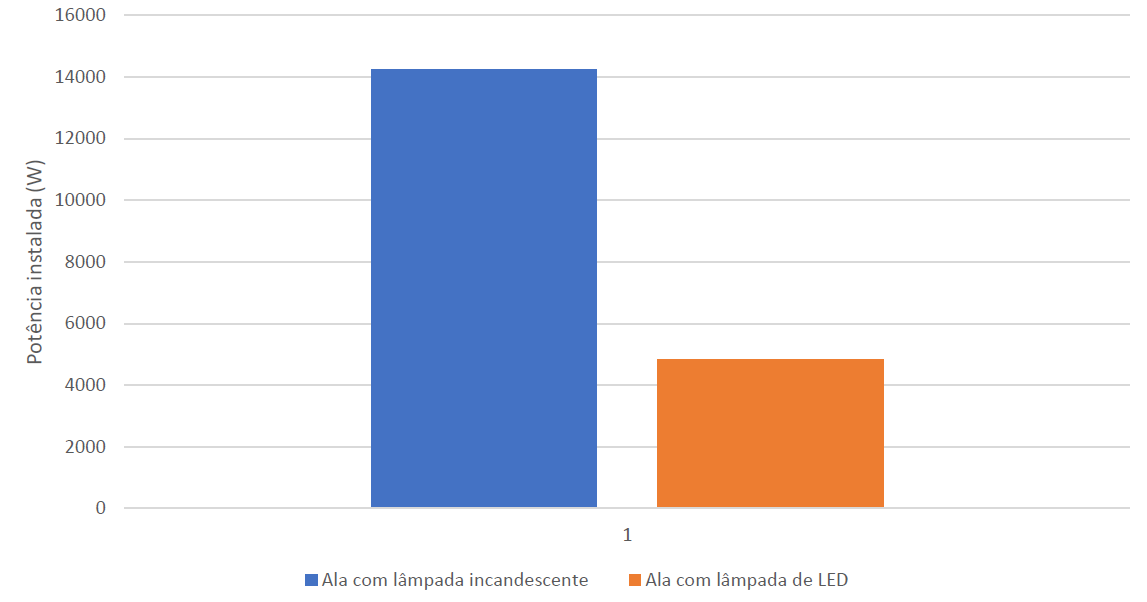
\includegraphics[width = 1.1\textwidth]{Figuras/graph2.PNG}
\caption{Gráfico da comparação entre os valores da potência atual instalada das alas que usam lâmpadas incandescentes e de LED.}
\label{graph2}
\end{figure}


Ao substituir todas as lâmpadas da edificação, por lâmpadas de LED com potência de 18 W, tomando como base as lâmpadas já instaladas na edificação, com luminárias, que utilizam apenas 2 lâmpadas, tem-se uma redução significativa da potência instalada da edificação, conforme mostra a Tabela \ref{tab_proj}.

\begin{table}[H]
\centering
\caption{Tabela de projeções da potência instalada com a alteração sugerida.}
\label{tab_proj}
\begin{tabular}{ll}\hline  
Pavimento          & \begin{tabular}[c]{@{}l@{}}Potência instalada\\   (W)\end{tabular} \\\hline  
Pavimento Térreo   & 7164                                                               \\
Segundo Pavimento  & 8388                                                               \\
Terceiro Pavimento & 10044                                                              \\\hline  
Total              & 25596                \\\hline                                               
\end{tabular}
\end{table}
O gráfico da Figura \ref{graph1} mostra uma comparação entre potência instalada por pavimento, e a potência total, com o valor da potência que cada pavimento teria, e o total também, com a substituição por lâmpadas de LED, com potência de 18 W. Nota-se que a potência da projeção, é muito menor, que a instalada, sendo que a potência total da projeção representa cerca de 45\% do valor da potência atual instalada, ou seja, a potência será reduzida em torno de 55\% do valor atual.

\begin{figure}[H]
\centering
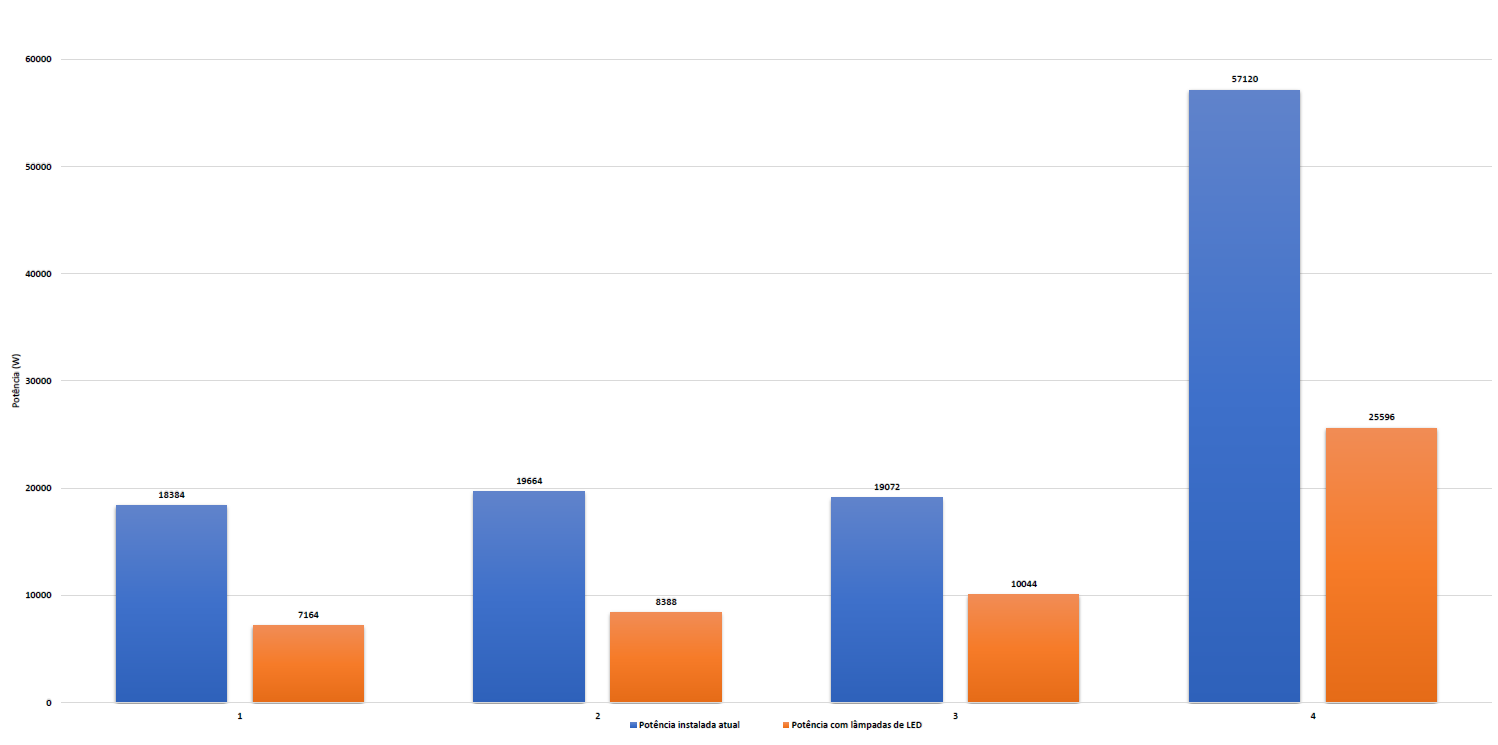
\includegraphics[width = 1.1\textwidth]{Figuras/graph1.PNG}
\caption{Gráfico da comparação entre os valores da potência atual instalada, e a potência de projeção com a alteração sugerida.}
\label{graph1}
\end{figure}


Por pavimento, pode-se observar que, no pavimento térreo, a potência da projeção representa cerca de 39\% da potência atual instalada, sendo reduzida em torno de 61\% ao instalar as lâmpadas de LED. Para o segundo pavimento, a redução é de cerca de 57\%, e para o terceiro pavimento, a redução é de 47\%.

Os valores percentuais de redução da potência instalada variam por pavimento, devido à alguns fatores:
\begin{itemize}
\item No pavimento térreo, grande parte do edifício ainda utiliza lâmpadas incandescentes com potência de 40 W, e luminárias que utilizam 4 lâmpadas, o que resulta em uma grande potência instalada, o que justifica esse alto índice de redução, com a projeção de instalação de lâmpadas de LED;
\item No segundo pavimento, mesmo com uma ala já possuindo a instalação de lâmpadas de LED, a outra ala, como já foi mostrado um comparativo anteriormente, utiliza lâmpadas incandescentes com potência de 40 W, e luminárias que utilizam 4 lâmpadas, o que justifica esse índice de redução;
\item No terceiro pavimento, por ser uma parte da edificação que foi construída após a reforma, conforme foi dito anteriormente, as lâmpadas instaladas são fluorescentes, com uma potência de 32 W, e já possue luminárias que utilizam apenas 2 lâmpadas, e portanto, possue menor índice de redução. 
\end{itemize}

A implementação dessa solução de melhoria, teria um custo, de certa forma, elevado, uma vez que as lâmpadas de LED, possuem um valor elevado, quando comparados aos custos das lâmpadas incandescentes e fluorescentes. Porém, o investimento vale a pena, tendo em vista que, ao longo prazo, esse investimento será compensado no custo do consumo energético da edificação. O sistema de iluminação será muito mais eficiente, o que gerará uma economia no consumo energético, e consequentemente, uma economia no gasto com energia elétrica.

Para atender aos outros pré-requisitos para o sistema de iluminação, previstos no RTQ-C, vê-se necessário, a instalação de um dispositivo de controle, para desligar automaticamente, o sistema de iluminação. A alternativa viável para atender esse critério, seria a implantação de sensores de presença, nos corredores da edificação, uma vez que, no período noturno, a iluminação dos corredores permanece ligada de forma constante, até encerrar toda as atividades do edifício. Esse dispositivo seria programado para desligar o sistema de iluminação após 30 minutos após a saída de todos os ocupantes, conforme prevê o RTQ-C, e ligaria a iluminação ao detectar a presença de alguma pessoa no ambiente. Nos demais ambientes da edificação, não se faz necessário essa implementação, tendo em vista, que as salas de aulas, quando não estão em atividade, o sistema de iluminação não permanece ligado.

Um ponto importante que pode ser melhor utilizado é a questão da luz natural. A luz natural, é um recurso muito importante, que ao ser utilizado de forma correta, gera uma grande economia no consumo de energia elétrica. Uma alteração importante a ser implementada na edificação, é um dispositivo de controle independente, para desligar a fileira de lâmpadas que se localizam próximas à janela. Uma opção interessante, para aproveitar melhor a luz natural nos ambientes, seria a implementação de um sistema de dimerização, que permite ajustar a intensidade luminosa das lâmpadas, podendo assim, ponderar a luz natural que entra no ambiente, com o sistema de iluminação, deixando o ambiente com uma iluminação agradável. Vale a pena ressaltar que, para cumprir ao critério da luz natural, é necessário, além do que foi descrito, realizar o método da simulação.

A implementação das sugestões realizadas, para melhorar a eficiência energética da edificação, apesar de ter um custo elevado, tornaria o edifício mais eficiente, tendo em vista os resultados obtidos do trabalho realizado em campo, ponderando com o resultados das projeções realizadas, a edificação, passaria a atender a todos os pré-requisitos, previstos para o sistema de iluminação no RTQ-C, e como a potência instalada no edifício já é abaixo da potência limite para o nível A, e como mostra as projeções, ainda teria uma redução de 55\% do valor total instalado atualmente, credenciaria a edificação a obter um ENCE parcial para o sistema de iluminação de nível A.



















		          % Capítulo 4 - Texto do cap4.tex
%%
\chapter{Discussões e Conclusões}\label{chp:conclusao}
\vspace{-1.5cm}
\noindent\rule{\columnwidth}{1.2mm}
\vspace{0.1cm}

O estudo apresentado, avaliou o sistema de iluminação, de uma edificação já existente, o Centro de Tecnologia e urbanismo da UEL, através do programa brasileiro de etiquetagem, tomando como base o regulamento técnico da qualidade para edificações Comerciais, de Serviço e Públicas, propôs melhorias necessárias para o alcance do nível A, na ENCE parcial do sistema de iluminação. Primeiramente, analisou-se o nível energético da edificação, e posteriormente, com as melhorias apresentadas, o impacto gerado por estas, na eficiência energética do edifício.

A edificação estudada, mostrou-se, no que diz respeito ao sistema de iluminação, muito eficiente, com base nas potências instaladas, o que surpreendeu positivamente, tendo em vista que uma parcela do edifício é uma construção antiga. No entanto, a classificação da ENCE parcial, foi penalizada, uma vez que a edificação não atende em sua totalidade, ao pré-requisitos específicos do sistema de iluminação, previstos no RTQ-C, que a credenciaria a uma ENCE de nível C. Porém como a edificação, mostrou-se eficiente ao realizar o método da área do edifício, foi necessário fazer uma ponderação, e a edificação recebeu uma classificação de nível B. Com as alterações sugeridas, é possível reverter essa situação, e assim a edificação, será credenciada a receber o nível A, na ENCE parcial do sistema de iluminação.

Com relação a análise das potências instaladas, as alterações sugeridas, mostram que é possível, reduzir esse valor em cerca de 55\% do valor atual instalado, tornando a edificação, que já mostra um valor aceitável, mais eficiente, reduzindo muito, o custo com energia elétrica, o que faz com que o investimento a ser realizado para a implementação, seja compensado à longo prazo.

O aproveitamento da luz natural, na edificação é um ponto importante a ressaltar, a alternativa de implementação de um sistema de dimerização, mostra-se muito interessante, tendo em vista, que com ele, é possível ter um bom aproveitamento da luz natural, e seu investimento, ao longo prazo acaba sendo compensado, com a redução dos gastos com energia elétrica pela edificação. É importante frisar que, para atender a este critério do RTQ-C, é necessário realizar o método da simulação.

Por fim, vale a pena ressaltar que o método prescritivo foi estabelecido como um conjunto de regras gerais para identificar a eficiência do
edifício e aplica-se à grande maioria de tipologias construídas atualmente no país. No entanto, ela não abrange todas as soluções possíveis de existir
em um edifício, e muitos casos só poderão ser avaliados pela simulação. Esta, por sua vez, pode incluir soluções que promovem a eficiência
energética e que não foram incluídas no método prescritivo, como aproveitamento da luz natural.



\vspace{-0.5cm}

\section{Trabalhos Futuros}

Esse trabalho, considerou apenas o sistema de iluminação, para o Centro de Tecnologia e Urbanismo da UEL. Assim, poderia ser realizado, futuramente, um estudo sobre os outros dois sistemas a serem avaliados no programa de etiquetagem brasileiro, a envoltória, e o sistema de condicionamento de ar. Neste caso, além de determinar o nível energético parcial de cada sistema, ou da edificação toda, poderia ser apresentadas sugestões para elevar esse nível energético.

Um outro estudo interessante que poderia ser realizado futuramente, é utilizar o método da simulação, tendo em vista que neste trabalho foi utilizado o método prescritivo, para poder realizar uma comparação entre os dois métodos, na obtenção da ENCE. 

				      % Capítulo 5 - Texto do cap5.tex
%%
%% Insira ou retire quantos capítulos desejar
%%--------------------------------------------------------------------------------------------


%----- Elementos Pós-Textuais--------------------------
%
%--------Referências-------------------------------------------------------------------------
\postextual
\bibliography{bibliografia_teste} % arquivo bibtex com as referências (modelo.bib)


%%--------Apendice-------------------------------------------------
%\apendice                  % Comando que inclui os apendices (sua autoria)
%%
%\include{apendice_1}				  % Apendice 1 - arquivo apendice_1.tex
%%
%\include{apendice_2}         % Apendice 2 - arquivo apendice_2.tex
%%
%% Descomente caso exista a necessidade da inclusão de apendices
%%---------------------------------------------------------------

%%--------Anexos-------------------------------------------------
\anexos                    % Comando que inclui os anexos (outros autores)
%%
\chapter{Limite máximo aceitável de densidade de potência de iluminação ($DPI_L$) para o nível de eficiência pretendido – Método das atividades do edifício.}
\begin{figure}[H]
\centering
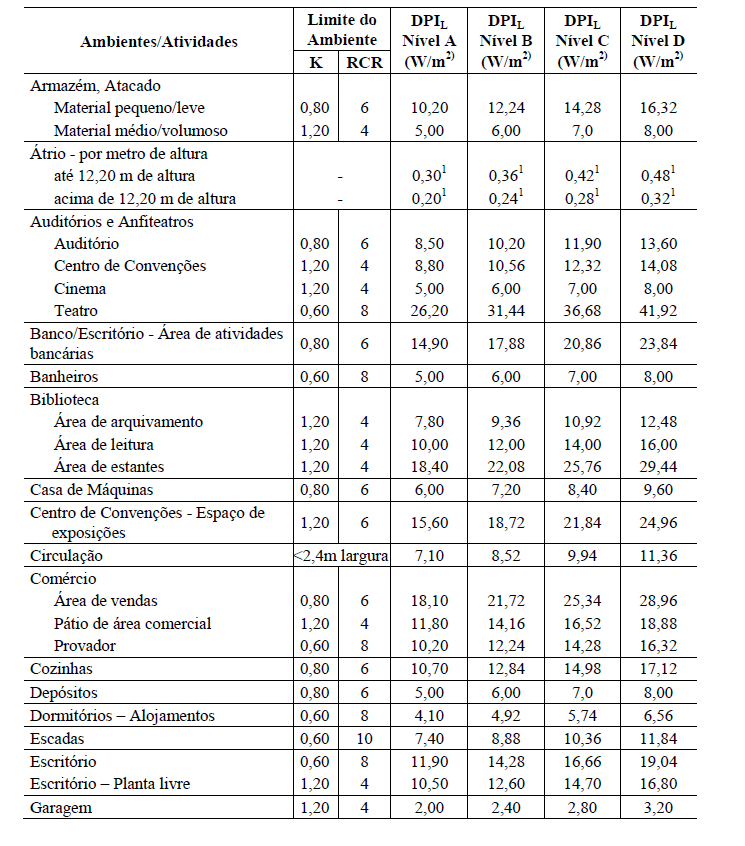
\includegraphics[width = 0.9\textwidth]{Figuras/tab1_1.PNG}
\caption{Limite máximo aceitável de densidade de potência de iluminação ($DPI_L$) para o nível de eficiência pretendido – Método das atividades do edifício.}
\label{tab2_1}
\textbf{Fonte:} Retirado de \cite{RTQ-C}.
\end{figure}

\begin{figure}[H]
\centering
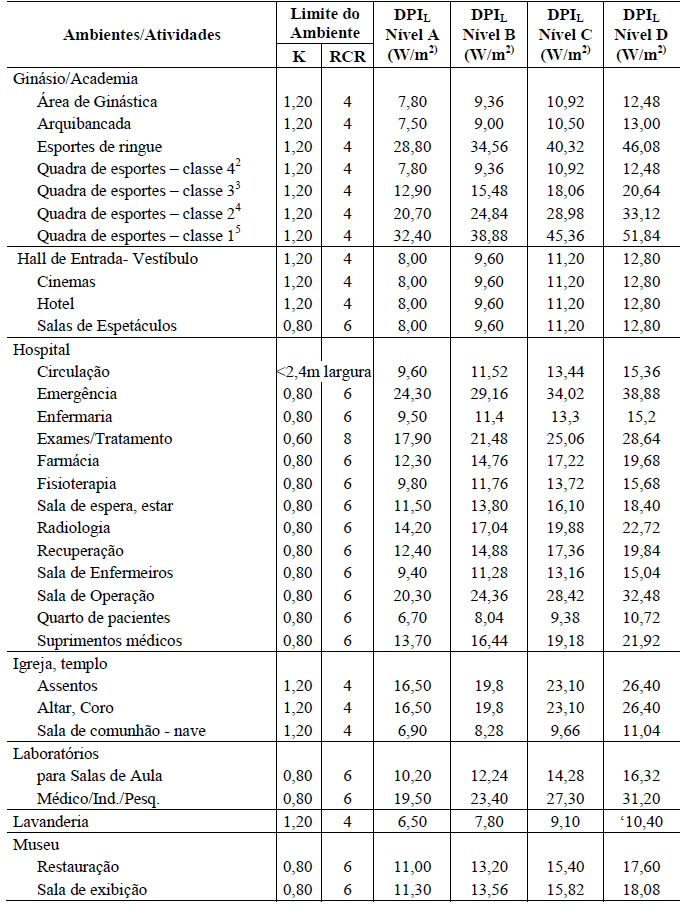
\includegraphics[width = 1.1\textwidth]{Figuras/tab1_2.PNG}
\caption{Limite máximo aceitável de densidade de potência de iluminação ($DPI_L$) para o nível de eficiência pretendido – Método das atividades do edifício(continuação).}
\label{tab2_2}
\textbf{Fonte:} Retirado de \cite{RTQ-C}.
\end{figure}

\begin{figure}[H]
\centering
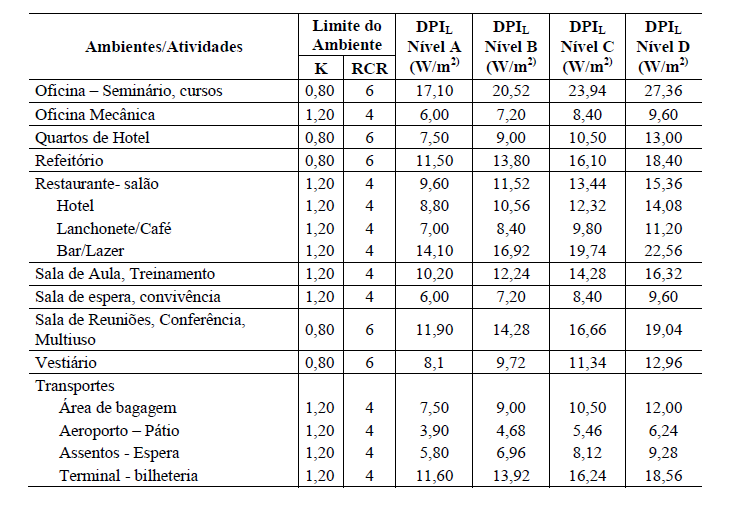
\includegraphics[width = 1.1\textwidth]{Figuras/tab1_3.PNG}
\caption{Limite máximo aceitável de densidade de potência de iluminação ($DPI_L$) para o nível de eficiência pretendido – Método das atividades do edifício(continuação).}
\label{tab2_3}
\textbf{Fonte:} Retirado de \cite{RTQ-C}.
\end{figure}





				  % Anexo 1 - arquivo anexo_1.tex
%%
%\include{anexo_2}          % Anexo 2 - arquivo anexo_2.tex
%%
%% Descomente caso exista a necessidade da inclusão de anexos
%%---------------------------------------------------------------

\end{document}
